\documentclass[12pt]{article}
\usepackage[utf8]{inputenc}
\usepackage{blindtext}
\usepackage{quotchap}
\usepackage{graphicx}
\setlength{\parindent}{12pt}
\setlength{\parindent}{0cm}
\usepackage[catalan]{babel}
\usepackage{enumerate}
\usepackage{float}
\usepackage{lmodern}
\newtheorem{theorem}{Teorema}
\usepackage{amsfonts}
\usepackage{url}


%Definició de la ela geminada per tal que accepti el punt volat del teclat
\def·#1{%
  \ifmmode
    \cdot #1
    %\csname normal@char\string"\endcsname l%
  \else%
    \def\argument{#1}%
    \if\argument l%
      \leftllkern=0pt\rightllkern=0pt\raiselldim=0pt%
      \setbox0\hbox{l}\setbox1\hbox{l\/}\setbox2\hbox{.}%
      \advance\raiselldim by \the\fontdimen5\the\font
      \advance\raiselldim by -\ht2%
      \leftllkern=-.25\wd0%
      \advance\leftllkern by \wd1%
      \advance\leftllkern by -\wd0%
      \rightllkern=-.25\wd0%
      \advance\rightllkern by -\wd1%
      \advance\rightllkern by \wd0%
      \allowhyphens\discretionary{-}{l}%
      {\hbox{}\kern\leftllkern\raise\raiselldim\hbox{.}
        \kern\rightllkern\hbox{l}}\allowhyphens%
    \else
      \if\argument L%
        \leftllkern=0pt\rightllkern=0pt\raiselldim=0pt%
        \setbox0\hbox{L}\setbox1\hbox{L\/}\setbox2\hbox{.}%
        \advance\raiselldim by .5\ht0%
        \advance\raiselldim by -.5\ht2%
        \leftllkern=-.125\wd0%
        \advance\leftllkern by \wd1%
        \advance\leftllkern by -\wd0%
        \rightllkern=-\wd0%
        \divide\rightllkern by 6%
        \advance\rightllkern by -\wd1%
        \advance\rightllkern by \wd0%
        \allowhyphens\discretionary{-}{L}%
        {\hbox{}\kern\leftllkern\raise\raiselldim\hbox{.}%
           \kern\rightllkern\hbox{L}}\allowhyphens%
      \else
        #1
      \fi
    \fi
  \fi
  }

\begin{document}

\pagestyle{empty}
\begin{titlepage}

\begin{center}
\vspace*{-1in}
\begin{figure}[htb]
\begin{center}

\includegraphics[width=10cm]{uab-mates_logo.png}
\end{center}
\end{figure}

FACULTAT DE CIÈNCIES\\
\vspace*{0.15in}

\begin{large}
TREBALL DE FINAL DE GRAU:\\
\end{large}
\vspace*{0.4in}
\begin{Large}
\textbf{Comparació de Xarxes Neuronals i algoritmes Random Forest per predir ingressos a la UCI de l'Hospital Clínic per COVID-19 } \\
\end{Large}
\vspace*{0.4in}
\begin{large}
Jaume Betriu i Tort\\
\end{large}
\vspace*{0.3in}
\rule{80mm}{0.1mm}\\
\vspace*{0.3in}
\begin{large}
Supervisat per: \\
Roger Borràs\\
\end{large}
\vspace*{1.4in}
Juliol, 2022
\end{center}

\end{titlepage}
\newpage

\pagenumbering{Roman} % per començar la numeració de pàgines en números romans
\pagestyle{plain}

\section*{Agraïments}
Agraeixo a la universitat i, en especial, al meu tutor Roger Borràs la formació que se'm ha procurat durant tots els meus anys de carrera i a l'ajuda rebuda per l'elaboració d'aquest projecte.

\newpage

\section*{Resum}
L'objectiu d'aquest projecte és dissenyar i entrenar un model de Machine Learning capaç de predir la probabilitat que un pacient desenvolupi simptomatologia greu i hagi de ser ingressat a la unitat de cures intensives per una infecció de COVID-19. El projecte es pot dividir en quatre blocs. El primer consisteix en un estudi teòric dels models de Deep Learning anomenats Xarxes Neuronals i dels models basats en arbres de decisió Random Forest. En el segon es fa un anàlisi de les dades que utilitzarem per entrenar els models. Aquestes dades recullen informació com pes, edat, malalties, gènere i altres variables referents a pacients positius de COVID-19 de l'Hospital Clínic de Barcelona. També es recull la variable a predir UCI que determina si aquell pacient va haver de ser ingressat a la unitat de cures intensives a causa de la malaltia. La tercera consisteix en l'entrenament de diverses Xarxes Neuronals i algoritmes Random Forest usant diferents hiperparàmetres i estructures. Per acabar, en l'última part es comparen els resultats i els models i s'exposen les conclusions del projecte.

\section*{Paraules clau}
Aprenentatge Profund, Aprenentatge Automàtic, Xarxes Neuronals, Arbres de decisió, COVID-19, Coronavirus.

\section*{Abstract}
This project's objective is the design and training of a Machine Learning model with the capability of predicting the probability of developing severe symthoms and having to be admitted to the intensive care unit of a hospital in the event of COVID-19 infection for a certain patient. We can divide the project into 4 main parts. The first section will concentrate on the theoretical development of Deep Learning models known as Neural Networks and tree-based models Random Forest. The second part consists of an analysis of the data that will train the models. This data contains information on weight, age, diseases, gender, and other variables related to positive COVID-19 patients from the Hospital Clínic de Barcelona. The data also contains the variable that we are interested in predicting, called UCI, that determines if the patient had to be admitted to the intensive care unit because of the infection. The third is the training of diverse Neural Networks and Random Forest models using different hyperparameters and structures. In the last part, we do a comparison of the results and the models, and we present our conclusions.

\section*{Index terms}
Deep Learning, Machine Learning, Neural Networks, Decision trees, Random Forest, COVID-19, Coronavirus.

\newpage

\tableofcontents

\newpage

\setcounter{page}{1} % reiniciar la numeració de pàgina
\pagenumbering{arabic} % canviar la numeració a números aràbics
\pagestyle{headings}

\section{Introducció i objectius del projecte}

L'objectiu principal d'aquest projecte és crear un model d'aprenentatge automàtic que pugui ser utilitzat per hospitals per detectar aquells pacients que siguin més propensos a desenvolupar simptomatologia greu derivada d'una infecció per COVID-19. És important remarcar que prioritzarem que el nostre model aconsegueixi detectar amb una precisió tan alta com sigui possible aquells pacients que no hauran de ser ingressats a l'UCI sacrificant, si fa falta, la precisió en aquells que sí per una raó obvia: Si el model ens retorna que un pacient patirà simptomatologia greu i es procedeix al monitoratge d'aquest, però finalment no desenvolupa aquests símptomes simplement se li donarà l'alta i no hi haurà més conseqüències. Per altra banda, si el model ens retorna que un pacient no patirà simptomatologia greu no se li farà cap monitoratge. El problema apareixerà si, en contra del pronòstic del model, el pacient acaba desenvolupant símptomes greus de la malaltia sense una preparació prèvia que podria tenir conseqüències fatals. \\

Per assolir aquest objectiu farem un estudi profund teòric de dos conjunts de models d'intel·ligència artificial: Els models de Deep Learning coneguts com a Xarxes Neuronals i els models basats en arbres de decisió Random Forest. Anirem des de les definicions més elementals fins a la formalització matemàtica d'aquests i, amb l'ajuda de les llibreries de Python PyTorch i H2O, utilitzarem aquests algoritmes per dissenyar i desenvolupar els models amb dades reals de pacients de l'Hospital Clínic de Barcelona. \\

Per acabar compararem els resultats dels dos models, estudiarem els seus comportaments i usarem el millor per fer prediccions sobre les nostres dades.

\newpage

\section{Intel·ligència artificial, Machine i Deep Learning}
Abans de parlar de Deep Learning, neurones, xarxes neuronals, funcions d'activació... (nocions que més endavant estudiarem en profunditat) cal parlar del conjunt que engloba tots aquests conceptes: La intel·ligència artificial. \\

Una manera ràpida i concisa per definir el que és la intel·ligència artificial (IA) és el següent enunciat:

\begin{quote}
\textit{La intel·ligència artificial es l'esforç d'automatitzar tasques intel·lectuals normalment portades a terme per humans}
\qauthor{François Chollet, \textit{Deep Learning with Python}}
\end{quote}

Com ja hem comentat la IA és un conjunt que conté els subconjunts Machine Learning i Deep Learning i aquests dos estan relacionats entre ells tal com mostra la següent figura:

\begin{figure}[H]
\centering
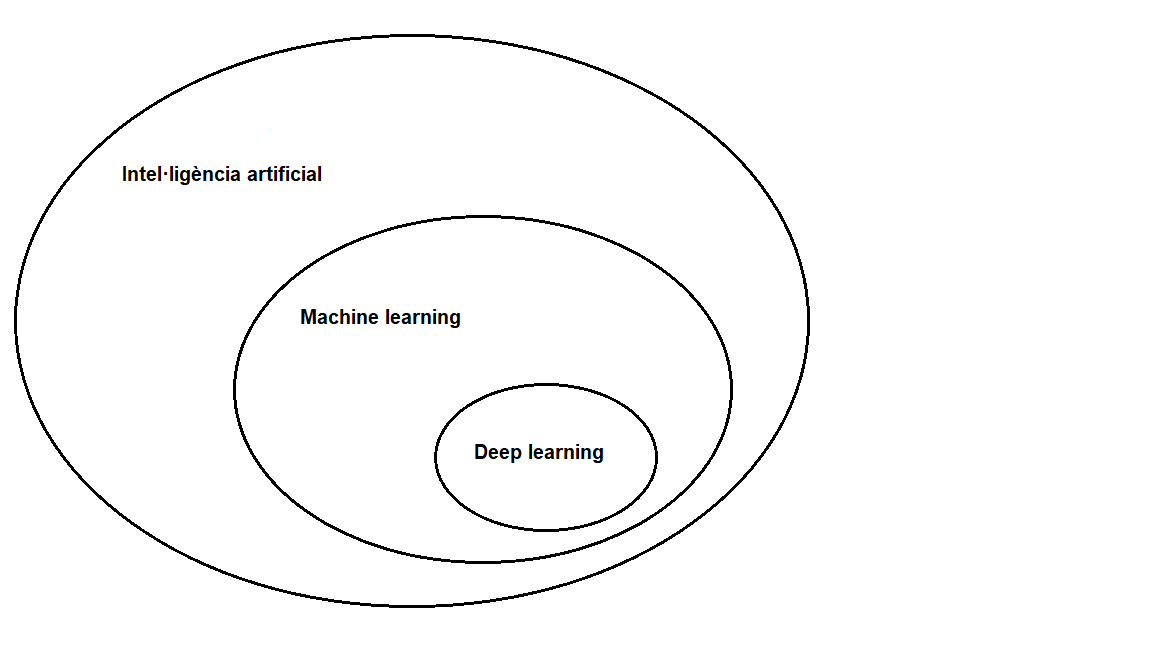
\includegraphics[scale=0.45]{relacio IA.png}
\label{fig: TDD}
\caption{Relació entre Deep Learning, Machine Learning i Intel·ligència artificial}
\end{figure}

 
Per tant, com podem apreciar en la figura, no tots els procediments inclosos en el camp de la IA inclouen algun tipus d'aprenentatge. Per posar un exemple els primers programes que jugaven a escacs estaven dissenyats a partir de regles implementades per programadors i durant un període considerable de temps es va creure que es podria assolir la fita d'una IA amb capacitat de raonament quasi humana mitjançant un conjunt prou gran de regles explicites dissenyades pels desenvolupadors. Aquest enfocament s'anomena IA simbòlica i va dominar el camp de la intel·ligència artificial des de la dècada dels 50 fins als 80.

Lamentablement, tot i que les IA simbòliques van donar resultats prou satisfactoris en problemes com jugar a escacs, a poc a poc aquest enfocament va quedar obsolet en ser intractables per resoldre problemes com la classificació d'imatges, el reconeixement de veu i la traducció entre d'altres. Va ser doncs quan un nou enfocament va començar a agafar força: El machine learning, o per la seva traducció: Aprenentatge Automàtic (AA).

\subsection{Machine learning o Aprenentatge Automàtic}

Pot una màquina anar més enllà del que ha estat explícitament programada per portar a terme? Podria un algoritme aprendre automàticament a força d'alimentar-lo amb dades? Un ordinador ens pot arribar a sorprendre? \\

Aquestes preguntes ens introdueixen a un nou camp dins la IA, l'Aprenentatge Automàtic. Com ja hem comentat, en els programes de IA simbòlics els programadors introdueixen una sèrie de regles i dades que seran processades utilitzant aquestes regles per extreure respostes. En canvi, en Aprenentatge Automàtic el programador introdueix les dades i també les respostes lligades a aquestes dades per tal que l'algoritme ens doni com a resultat les regles. Aquestes regles més endavant les podem aplicar a noves dades per tal d'obtenir noves respostes. La següent figura explica esquemàticament aquest fet:

\begin{figure}[H]
\centering
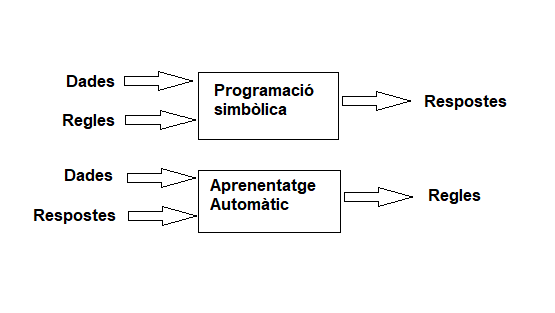
\includegraphics[scale=0.9]{Esquema AA.png}
\label{fig: TDD}
\caption{Esquema AA}
\end{figure}

Podríem dir que els sistemes AA són entrenats més que no pas programats explícitament. La idea principal és que se li presenten al sistema una sèrie d'exemples associats amb una resposta i l'algoritme troba una estructura estadística que permetrà al sistema deduir aquestes regles per fer prediccions amb noves dades.

Per exemple podríem entrenar un model d'AA amb un conjunt de fotografies de gats i gossos etiquetades a mà per un humà. Una vegada entrenat el model podríem comprovar com és de bo utilitzant un conjunt d'imatges de test (que no s'han fet servir per entrenar el model) i verificant que l'etiqueta que els hi associa el model siguin les correctes. Dependrà de diversos factors que aquest model sigui bo o no per la tasca per la qual l'hem entrenat, com ara que el conjunt d'exemples per l'entrenament sigui prou gran, que l'estructura estadística del model sigui adequada per la labor en qüestió, que no l'haguem sobreajustat a les dades d'entrenament i d'altres factors que discutirem durant el desenvolupament del projecte.

Resumint: per crear un model i fer Aprenentatge Automàtic necessitem en essència dos ingredients:

\begin{itemize}
    \item Dades d'entrada per entrenar el model. En el cas que hem presentat abans aquestes dades serien les fotografies dels gats i els gossos prèviament etiquetades de forma manual.
    \item Una manera de mesurar si l'algoritme està fent una bona feina a l'hora de classificar. Aquesta mesura s'utilitzarà per ajustar el model per tal que doni millors resultats com veurem més endavant.
\end{itemize}

Per tant, podríem dir que la paraula Aprenentatge (\textit{learning}) en aquest context descriu una mena de procés automàtic per trobar una representació millor de les dades.

\subsection{Introducció al Deep Learning}

Com ja hem comentat el Deep Learning (aprenentatge profund) és un subconjunt del Machine Learning. Un enfocament que posa èmfasi en nivells o capes d'aprenentatge ordenades successivament. La paraula deep (profund) no es refereix al fet que els models de Deep Learning gaudeixin d'un enteniment més profund de les qüestions, simplement fa referència a la idea d'ordenar diverses capes d'aprenentatge una rere l'altre per construir els models. La quantitat de capes que contribueixen en la construcció del model s'anomena la profunditat del model. \\

Considerem un primer exemple per posar una mica de llum a la qüestió: Suposem que volem dissenyar un algoritme que donada una imatge d'un nombre escrit a mà sigui capaç de saber quin és el nombre en qüestió. Un esquema de com un model de Deep Learning funcionaria és el següent:

\begin{figure}[H]
\label{fig: esquemaAA}
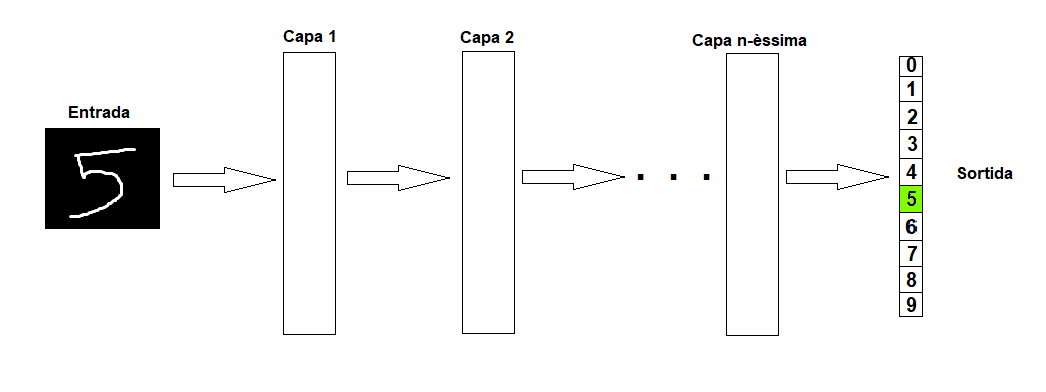
\includegraphics[scale=0.55]{esquema deep.png}
\caption{Esquema del funcionament dels models DL}
\centering
\end{figure}

Cada capa fa una sèrie de transformacions a certs paràmetres de les dades d'entrada i passa la informació a la següent capa. Podem pensar que aquesta informació va passant per diferents filtres i es va polint per tal que la informació de sortida sigui útil per, en el cas que estem considerant, classificar el nombre. Evidentment, aquestes transformacions no són aleatòries i, de fet, que el  model sigui prou bo per la tasca que li hem encomanat dependrà de com es fan. La idea doncs és que aquestes transformacions es facin d'acord amb els exemples d'entrenament que li hem donat al model. Quin tipus de transformacions es fan exactament i com es passa la informació de capa en capa ho estudiarem en profunditat en les següents seccions. 

En aquest projecte ens fixarem en les representacions en nivells anomenades xarxes neuronals, que són pràcticament el paradigma dominant en Deep Learning.

\newpage

\section{Xarxes neuronals}

Una xarxa neuronal és, tal com suggereix el seu nom, una sèrie de neurones interconnectades entre si i ordenades per nivells o capes. El primer nivell s'anomena nivell d'entrada (\textit{input layer} en anglès), l'últim nivell es coneix com a nivell de sortida (\textit{output layer}) i ens referirem als nivells intermedis com nivells ocults (\textit{hidden layers}). En el cas que entre dues capes successives (capa $n$ i capa $n+1$) totes les neurones de la cap $n$ estiguin connectades a totes les neurones de la capa $n+1$ direm que la xarxa és una xarxa neuronal totalment connectada. Però que és una neurona? Té alguna cosa a veure amb les neurones que tots coneixem? \\

Podríem dir que la resposta és que sí. D'ara endavant coneixerem com a neurona a un node que pren un valor (un \textit{input}) d'entrada, fa certes computacions per transformar aquesta entrada i expulsa un valor de sortida en dos passos:

\begin{itemize}
    \item Combinació de l'input o entrada
    \item Funció d'activació
\end{itemize}
seguint el següent esquema:

\begin{figure}[H]
\label{fig: esquemaNeurona}
\centering
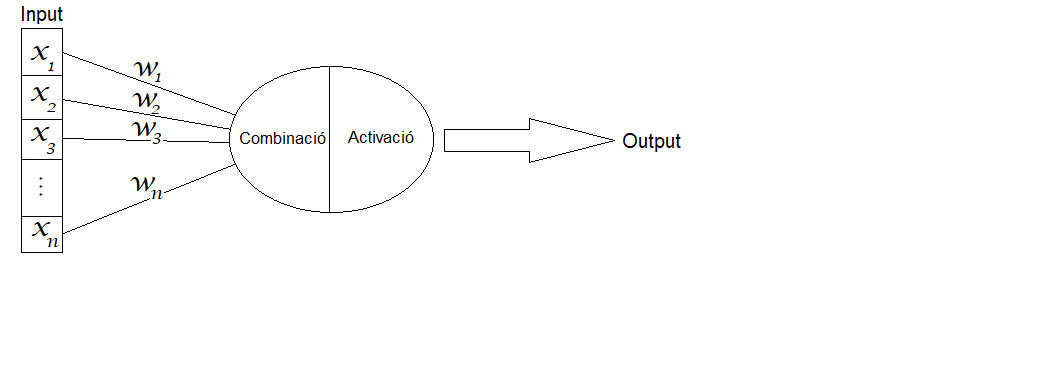
\includegraphics[width=18 cm, height = 7 cm]{esquema neurona.png}
\caption{Funcionament d'una neurona}
\end{figure}

Com podem veure el funcionament és molt senzill. Introduïm a la neurona una sèrie de dades en forma de input multiplicades per uns certs pesos ($w_1, \cdots,w_n$), combinem aquests valors i a continuació fem una transformació anomenada activació.

Anem per parts, com es fa aquesta combinació? Tenim diverses possibilitats que presentarem però la que més es fa servir és la primera:

\begin{itemize}
    \item Suma ponderada: $$z(x_1,\cdots,x_n)=\sum ^n_{i=1} w_i x_i$$
    \item Màxim o mínim: $$z(x_1,\cdots,x_n)=max(w_1 x_1,w_2 x_2,\cdots ,w_n x_n)$$
                         $$z(x_1,\cdots,x_n)=min(w_1 x_1,w_2 x_2,\cdots ,w_n x_n)$$
    \item Lògic AND($\wedge$)/OR($\vee$): (en cas de que l'input siguin valors binaris) $$z(x_1,\cdots,x_n)=w_1 x_1 \wedge w_2 x_2 \wedge \cdots \wedge w_n x_n$$
    $$z(x_1,\cdots,x_n)=w_1 x_1 \vee w_2 x_2 \vee \cdots \vee w_n x_n$$
\end{itemize}
Com ja hem comentat la més comuna és la suma ponderada i és la que utilitzarem d'ara endavant per defecte, en excepció dels casos que especifiquem que farem servir un altre tipus de combinació.

És comú també afegir al pas de combinació un element $b$ que anomenem biaix que és suma al resultat. Per exemple, en el cas de la suma ponderada l'afegiríem de la següent manera:

$$z(x_1,\cdots,x_n)=\sum ^n_{i=1} w_i x_i +b$$ 

\subsection{Funcions d'activació}
L'activació no és més que aplicar al valor que extraiem de la combinació una funció preestablerta. Existeixen un gran ventall de funcions d'activació i en aquest projecte utilitzarem les següents:

\begin{itemize}

    
\item \textbf{Funció sigmoide}:
    $$\sigma(x)=\frac{1}{1+e^{-x}}$$
    
\begin{figure}[H]
\label{fig: esquemaNeurona}
\centering
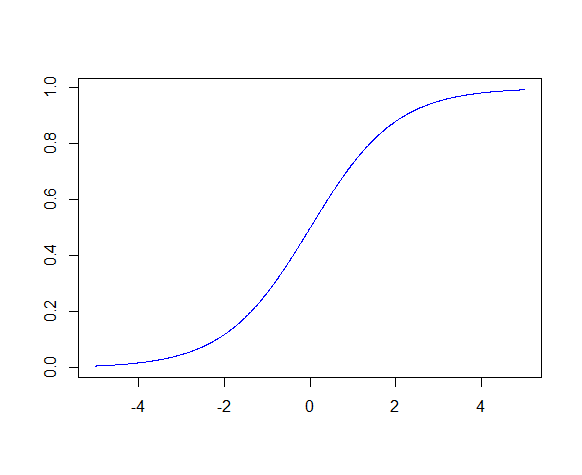
\includegraphics[scale=0.7]{Sigmoid gràfic.png}
\caption{Funció sigmoide}
\end{figure}

La mateixa funció que s'utilitza amb la regressió logística. Útil en el cas que ens interessi un output entre 0 i 1, per exemple en el cas de que l'output desitjat sigui una probabilitat. A diferència de la funció que ve a continuació, la sigmoide és diferenciable en tot punt.

\item \textbf{Funció ReLU:}
    $$f(x)=max(0,x)$$

\begin{figure}[H]
\label{fig: ReLU}
\centering
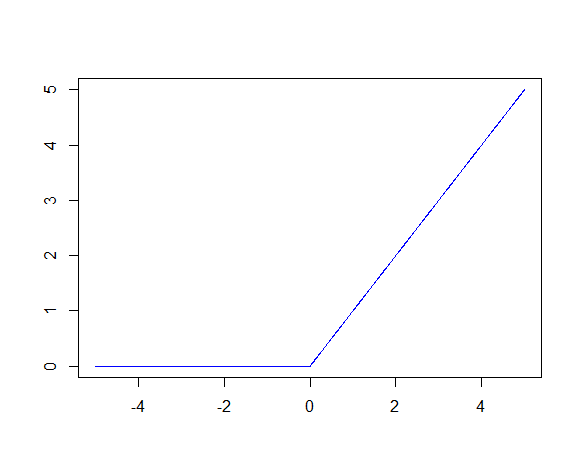
\includegraphics[scale=0.7]{relu.png}
\caption{Funció ReLU}
\end{figure}


Simple i sorprenentment molt útil a la pràctica, ja que el seu gradient és molt fàcil de calcular.

\item \textbf{Funció Softmax}

La funció Softmax és un cas especial de funció d'activació que combina l'output de diverses neurones de la mateixa capa.

Si posem $z_j$ com el resultat del pas de combinació de la neurona $j$ i considerem $z=(z_1, \cdots, z_K )$ on $K$ és la dimensió de la capa definim la funció Softmax com:

$$S(z)_j = \frac{e^{z_j}}{\sum ^K _{i=1} e^{z_i}} $$

Si ens fixem en la funció Softmax ens adonarem que si fem la suma de tots els ouptuts obtenim:

$$\sum _{i=1} ^{K} S(z)_i = 1$$ 

És lògic doncs pensar en els ouputs com la distribució de probabilitat entre $K$ possibles categories, molt útil en problemes de classificació com per exemple el cas ja mencionat dels nombres escrits a mà. 

\end{itemize}

Arribats a aquest punt ja sabem tots els elements que constitueixen una xarxa neuronal i les operacions que transformen els inputs en ouputs a mesura que avancen per les diferents capes. La pregunta doncs és com ens pot ajudar aquesta estructura a resoldre problemes? Quines condicions s'han de complir per tal que una xarxa neuronal pugui arribar a ser útil per tal d'afrontar reptes com el reconeixement d'imatges? 

En aquesta secció parlarem del nombre de neurones, de capes, funcions de cost i com optimitzar-les i de com podem utilitzar aquests conceptes a l'hora de dissenyar models predictius útils i funcionals. Començarem parlant de les dimensions de les xarxes.

\subsection{Profunditat, complexitat i estructura de les xarxes neuronals}

Seleccionar un nombre òptim de capes i un nombre òptim de neurones per cada una de les capes pot ser una labor força complicada. Per norma general afegir neurones a una capa concreta o afegir noves capes a una xarxa millorarà la capacitat predictiva del model, però cal matisar molt aquesta afirmació. És cert que una xarxa neuronal profunda (amb més capes) serà capaç de comprendre estructures molt més complexes i afegint neurones permetrem al model crear noves característiques basades en l'output de les capes anteriors, però cal anar amb compte i mantenir un equilibri entre complexitat i dimensió de les dades d'entrenament. \\

No hi han normes generals de com s'ha de definir l'estructura d'una xarxa neuronal però depenent de quin sigui el nostre objectiu les podem classificar en dos grans grups:

\begin{itemize}
    \item \textbf{Arquitectura per regressió: } En cas que el nostre objectiu sigui resoldre un problema de regressió ens decantarem per estructures on l'última capa de la xarxa consisteixi en una sola neurona, com per exemple:

\begin{figure}[H]
\label{fig: esquemaNeuronaReg}
\centering
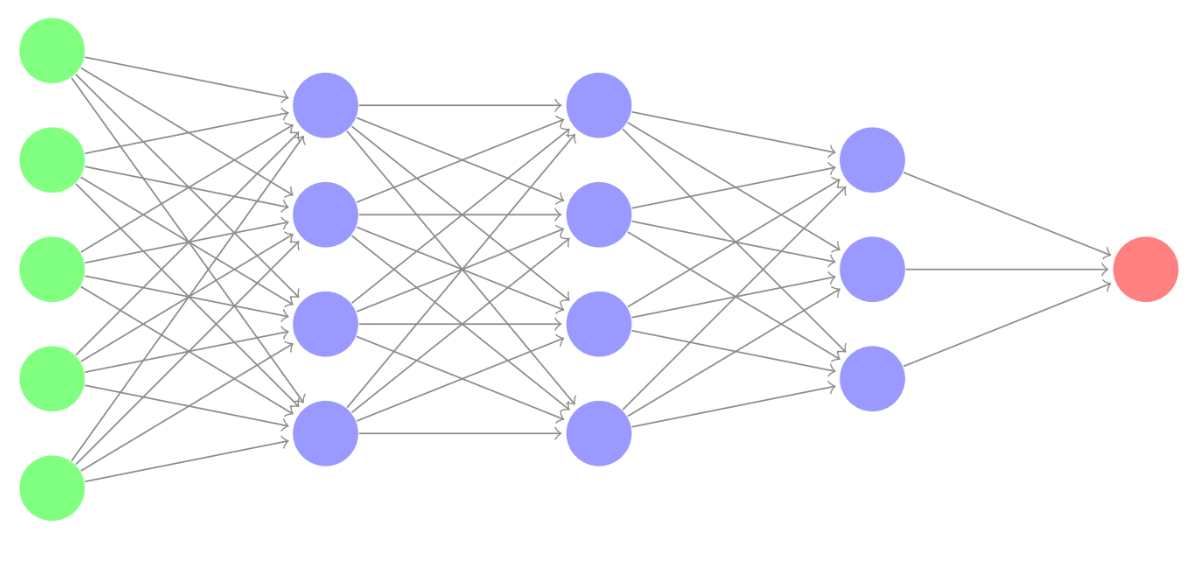
\includegraphics[scale=0.26]{regression_structure.png}
\caption{Arquitectura de regressió}
\end{figure}

    \item \textbf{Arquitectura per classificació: } Quan ens enfrontem a problemes de classificació és essencial que l'última capa de la nostra xarxa tingui el mateix nombre de neurones com classes tenim per classificar. A més a més, com ja hem comentat, és molt útil utilitzar l'activació Softmax en aquesta última capa en aquest cas. Un exemple seria:
    
\begin{figure}[H]
\label{fig: esquemaNeuronaClass}
\centering
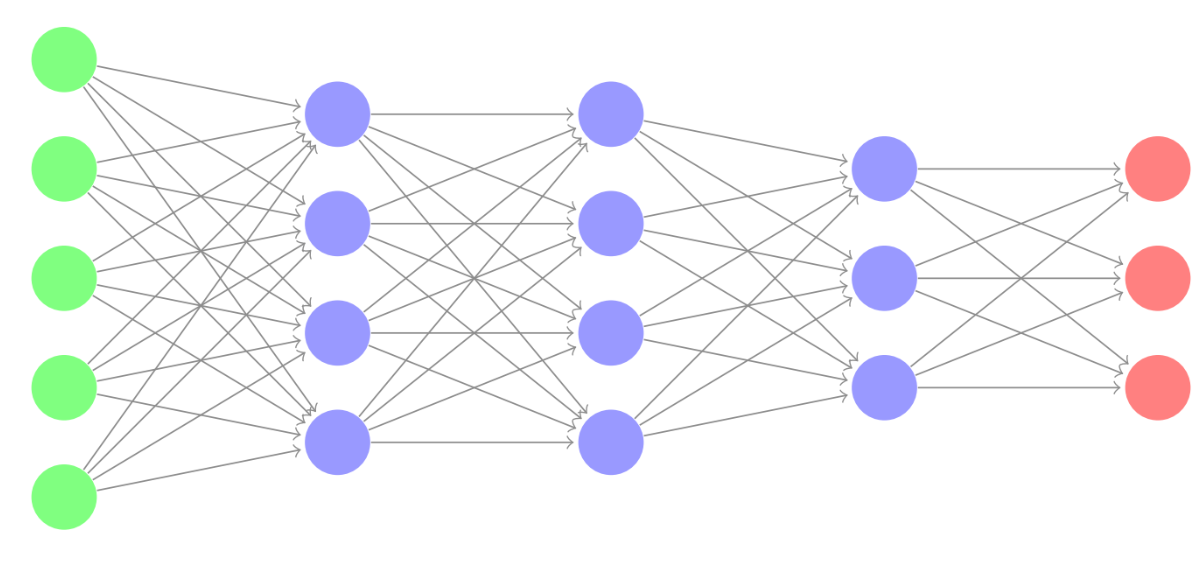
\includegraphics[scale=0.26]{classification_structure.png}
\caption{Arquitectura de classificació}
\end{figure}

\end{itemize}

Tot i això hem de tenir especial cura a l'hora de definir les dimensions de la nostra xarxa per tal d'evitar l'enemic número 1 dels models de AA: el sobreajustament. Parlarem en profunditat d'aquesta qüestió més endavant ja que és un dels problemes més recurrents a l'hora de crear models de Deep Learning.

\subsection{Funcions de cost, optimització i entrenament}

Com ja hem vist, cada neurona està constituïda per una combinació de l'input d'entrada al qual se li aplica tot seguit una funció d'activació. Aquesta primera combinació conté uns elements que hem anomenat pesos i el biaix:

$$(w_1, \cdots,w_n,b)$$

Elements que també reben el nom de paràmetres entrenables. Aquests elements contindran la informació que la xarxa ha anat aprenent a l'exposar-la a les dades d'entrenament. Per tal d'entrenar el model i adaptar-lo a les dades d'entrenament el primer pas és definir una manera de mesurar si el nostre algoritme és bo o no a l'hora de modelar aquestes. Llavors, d'alguna manera, el nostre objectiu serà aconseguir reduir al màxim aquests errors amb l'esperança que això ens permeti fer prediccions encertades amb noves dades. 

Per tal de desenvolupar més en profunditat aquest pas, cal que parlem d'un concepte fonamental. Les funcions de cost.

\subsubsection{Funcions de cost}

Les funcions de cost són funcions que ens ajudaran a mesurar com de bé (o com de malament) el nostre model fa prediccions dins les nostres dades d'entrenament. Podem trobar-ne de molts tipus diferents i depenent de si el nostre és un problema de regressió o de classificació haurem d'inclinar-nos per un tipus o un altre. Tot i així, totes comparteixen la mateixa estructura: \\

Suposem que hem creat un model $f$ que depèn d'uns paràmetres $w$ modificables. Suposem també que tenim un input $x$ el qual ens agradaria que el nostre model transformés en un output $y$. Llavors és raonable pensar en una manera de mesurar com de lluny està la predicció que fa el model $f$ amb l'input $x$ i el valor real $y$. És a dir, la funció de cost té la forma general:

$$L(w) = distància(f_w(x),y)$$

En el cas concret de les xarxes neuronals els paràmetres $w$ són els pesos i el biaix. Fixem-nos que com més petit sigui el valor de la funció, més a prop estaran les prediccions dels valors reals i més precís serà el nostre model. Vegem algunes funcions de cost típiques:

\begin{itemize}
    \item \textbf{Error quadràtic mitjà}
    
Si posem com $(y_1, \cdots, y_N)$ els valors reals a predir i $(\hat{y_1}, \cdots, \hat{y_N})$ les prediccions que ens retorna la xarxa definim l'error quadràtic mitjà com:

$$L_{MSE} = \frac{1}{N} \sum ^N _{i=1} (y_i - \hat{y_i})^2 $$

Molt utilitzada en problemes de regressió.

\item \textbf{Entropia creuada categòrica}

L'entropia creuada categòrica o funció de cost logarítmica s'utilitza en problemes de classificació. Considerem una xarxa amb $K$ neurones a l'última capa i l'output té l'activació Softmax. \\

Suposem també que volem fer $N$ prediccions per classificar $N$ instàncies entre $M$ categories. Suposem que per portar a terme tal labor dissenyem una xarxa neuronal amb $M$ neurones a l'última capa i activació Softmax. Per tant, per cada instància $i$ el model ens tornarà $M$ probabilitats $\hat{p_{ij}}$ on aquesta és la probabilitat d'assignar la categoria $j$ a la instància $i$. Llavors definim la funció de cost logarítmica com:

$$L_{log} = -\frac{1}{N} \sum ^N _{i=1} \sum ^M _{j=1} y_{ij} log(\hat{p_{ij}}) $$

On $y_{ij}$ és un indicador binari que és $1$ si la categoria $j$ és la correcta per la instància $i$ i $0$ en cas contrari. Notem que només els termes de la categoria correcta per cada una de les instàncies contribueixen a la suma i observem que un classificador perfecte tindria $L_{log} = 0$ i valors progressivament més grans indicarien classificadors menys exactes.
\end{itemize}

\subsubsection{Entrenament del model}

Com ja hem anat introduint, la manera d'entrenar una xarxa consistirà en modificar d'una manera concreta els pesos i biaixos del model per tal que modeli correctament les dades d'entrenament. Per tant, el procés d'entrenament consistirà en utilitzar un mètode iteratiu per anar refinant aquests paràmetres i a cada pas utilitzar la nostra funció de cost de preferència per testejar si hi ha hagut millora. És a dir, aquest pas consisteix en optimitzar la funció de cost respecte als paràmetres $w$ i $b$.  

Pensem un moment en la funció de cost $L$. Si analitzem les seves components ens adonarem que, com ja hem fet notar al definir-la, si tenim un número fixat $N$ d'instàncies en les nostres dades d'entrenament $L$ només depèn dels paràmetres $w, b$. És lògic doncs fer servir el gradient de la funció $L$ per tal de trobar un mínim d'aquesta. \\

És conegut que el sentit oposat a on apunta el gradient d'una funció en un punt indica la direcció i el sentit de màxim decreixement.  Per tant, la nostra estratègia podria ser utilitzar un algoritme iteratiu com el següent:

$$x_{t+1} = x_t - \eta \nabla_{x} L(x_t) $$

On $\nabla_{x} L(x_t)$ és el vector gradient de $L$ en el punt $x_t$ i $\eta$ és un paràmetre d'aprenentatge. \\

Aquest algoritme no ens assegura trobar el mínim global en casos no convexos, però pot ser molt útil per trobar mínims locals i amb cada iteració tenim l'esperança que el punt $x_t$ convergeixi cap a un d'aquests mínims. Posats en aquesta situació només ens cal aclarir un fet, com calculem el gradient $ \nabla_{x} L$?

\subsubsection{Backpropagation}

Tornant a l'exemple de la xarxa que hem posat per exemple al parlar de l'estructura de regressió si calculem el nombre de paràmetres entrenables (incloent-hi els biaixos) obtenim:

$$6·4 + 5·4 + 5·3 +4 = 63$$

És a dir, cal optimitzar $L$ en funció de $63$ paràmetres que a més a més han sofert composició de les funcions d'activació. Una labor pràcticament impossible i no escalable d'enfocar de la manera tradicional (calculant l'expressió de $L$ i derivant parcialment respecte a els seus paràmetres). Cal buscar un nou enfocament més eficient i el mètode de la Backpropagation (propagació enrere) és una bona solució. Abans de presentar-la, ens caldrà introduir una mica de notació i enunciar un teorema ja conegut per tots, la regla de la cadena:

\begin{theorem}[Regla de la cadena:] \\

Siguin $f$, $g$ funcions contínues sobre els reals d'una variable. Llavors la derivada de la composició $g(f(x))$ respecte $x$ satisfà:
$$\frac{\partial (g \circ f)}{\partial x} = \frac{\partial g}{\partial f} \cdot \frac{\partial f}{\partial x} $$
\end{theorem}

\textbf{Notació matemàtica:}

\begin{itemize}
    \item $n_l =$ Nombre de neurones a la capa $l$. Suposarem doncs que $n_0$ serà la dimensió de la primera capa i de l'input.
    
    \item $X \in M_{n_o \times m}(\mathbb{R})$ és la matriu que conté totes les instàncies. En un context de programació, és el nostre dataframe.
    
    \item $W^{[l]} \in M_{n_l \times n_{l-1}} (\mathbb{R})$ denota la matriu que conté els pesos que connecten la capa $l-1$ amb la capa $l$. \\
    Particularment l'element de la fila $j$, columna $k$ denotat per $w_{jk} ^{l}$ és el pes de la connexió entre la neurona j de la capa $l$ i la neurona $k$ de la capa $l-1$.
    
    \item $b^{[l]}$ és un vector de  mida $n_l$ que denota el biaix de la capa $l$. Els elements $b_j ^{[l]}$ denoten el biaix de la neurona $j$ en la capa $l$.
    
    \item $z^{[l]}$ és un vector de mida $n_l$ que conté la combinació de la capa $l-1$.
    
    \item $g$ la funció d'activació com ara la funció ReLU o sigmoide. \\
    Llavors si $S \in M_{c \times d} (\mathbb{R})$ denotarem per $g(M) \in M_{c \times d} (\mathbb{R})$ la matriu obtinguda a l'aplicar la funció $g$ component a component. El cas particular $d=1$ és la notació per vectors.
    
    \item Denotem $a^{[l]} \in M_{n_l \times 1} (\mathbb{R})$ l'output de la capa $l$. En particular en una xarxa amb $L$ capes denotem per $a^{[L]}$ l'output de la xarxa neuronal i per conveni $a^{[0]}$ el vector d'inputs.
    
\end{itemize}

Llavors tindrem:

$$z_j^{[l]}= \sum _{k=1}^{n_{l-1}} w_{jk}^{[l]} \cdot a_k^{[l-1]} + b_j^{[l]} $$
$$a_j^{[l]} = g(z_j^{[l]}) $$

o en forma matricial:

$$z^{[l]} = W^{[l]} \cdot  a^{[l-1]}+b^{[l]}$$
$$a^{[l]} = g(z^{[l]})$$

Aplicant de manera recursiva l'expressió anterior capa a capa obtindrem l'output de la xarxa $a^{[L]}$ i definirem l'error del model amb la funció $L(y,a^{[L]})$ on $y$ és la categoria correcta de l'exemple en el qual estem treballant. \\

Al cap i a la fi, com l'element $a^{[L]}$ depèn dels paràmetres $W^{[l]}$ i $b^{[l]}$ la funció de cost $L$ també dependrà d'aquests paràmetres. En conseqüència, modificant-los obtindrem resultats de $L$ diferents. El nostre objectiu doncs és el de minimitzar $L$ modificant aquests paràmetres utilitzant, com ja hem comentat, la regla de la cadena i el gradient amb el mètode de la Backpropagation (propagació cap enrere). Aquest algoritme consistirà en aplicar la regla de la cadena recursivament per anar calculant les derivades parcials de $L$ respecte tots els paràmetres. Posem un exemple: \\

Suposem que la nostra xarxa és un classificador binari. És a dir, el valor real esperat és o bé $1$ o bé $0$. Llavors si prenem com a funció de cost la logarítmica tindrem:

$$L(y, a^{[L]}) = -[y \cdot log(a^{[L]}) + (1-y) \cdot log(1-a^{[L]})] \Rightarrow \frac{\partial L}{\partial a^{[L]}} = - \left( \frac{y}{a^{[L]}} - \frac{1-y}{1-a^{[L]}}) \right) $$

Per tant, si volem calcular la derivada parcial de $L$ respecte $w^{[l]}_{jk}$ considerem els altres paràmetres com a constants i apliquem la regla de la cadena:

$$ \frac{\partial L}{\partial w^{[l]}_{jk}} = \frac{\partial L}{\partial a^{[l]}_j} \cdot \frac{\partial a_j ^{[l]}}{\partial z^{[l]}_j} \cdot \frac{\partial z_j ^{[l]}}{\partial w^{[l]}_{jk}}$$

Notem que per fer aquests càlculs cal saber els valors de $z^{[l]}$ i $a^{[l]} \ \forall l=1,\ldots,L$ que s'han calculat en el procés de calcular $a^ {[L]}$. Una vegada calculat el gradient podem recórrer a diferents mètodes iteratius per tal d'obtenir valors que minimitzin la funció de cost.

\subsubsection{Algoritmes d'optimització}

Ja hem comentat que una possible estratègia és utilitzar l'algoritme iteratiu

$$x_{t+1} = x_t - \eta \nabla_{x} L(x_t) $$

amb l'esperança que els punts $x_t$ convergeixin cap a un mínim global o local. Utilitzant aquest algoritme a cada pas calcularem el gradient de $L$ utilitzant el total de totes les dades disponibles. Aquest fet converteix en intractable aquest enfocament en la majoria de casos en què desitgem entrenar el nostre model amb grans datasets. Cal buscar altres variants més ràpides i eficients:

\begin{itemize}
    \item \textbf{Descens estocàstic del gradient}
    
    En aquest cas en comptes d'utilitzar el total de totes les nostres dades per calcular el gradient, utilitzarem una sola observació $v^i$ amb la seva respectiva classificació $u^i$ per calcular una aproximació del gradient:
    
    $$ x_{t+1} = x_t - \eta \nabla_{x} L(x_t /  v^i:u^i) $$
    
    Evidentment, aquest mètode és molt més ràpid, ja que només tenim en compte una sola observació, però, per altra banda, pot ser molt inestable i no convergir de manera correcta.
    
    \item \textbf{Descens en mini-batches del gradient}
    
    És lògic que l'opció més utilitzada sigui un punt entremig entre els dos algoritmes anteriors, buscant rapidesa i estabilitat al mateix temps. Un batch de mida $n$ és un subconjunt del total de les dades amb $n$ observacions i utilitzarem aquest batch per calcular una aproximació del gradient de la següent manera:
    
    $$ x_{t+1} = x_t - \eta \nabla_{x} L(x_t /  v^{i : i+n}:u^{i : i+n}) $$
    
    On ${v^{i : i+n}:u^{i : i+n}}$ és el batch de mida $n$. És comú que el valor de $n$ prengui valors en el rang de $50$ fins a $256$. Definirem un EPOC com una iteració completa de l'algoritme.
\end{itemize}

El principal problema que ens trobem amb aquests algoritmes és que poden quedar-se atrapats en mínims locals. És per això que s'utilitzen variants del descens per gradient tradicional per augmentar la velocitat de convergència i evitar l'estancament:

\begin{itemize}

    \item \textbf{Mètode del moment}
    
    El mètode del moment consisteix en utilitzar el gradient de les iteracions anteriors multiplicat per una constant per tal de determinar la direcció:
    
    $$y_t = \beta y_{t-1} + \eta \nabla_{x} L(x_t) $$
    $$x_{t+1} = x_t - y_t$$
    
    On $\beta$ és el moment i se li acostuma a donar un valor al voltant de $0.9$. Aquesta millora ens permetrà tractar amb gradients molt petits però amb un preu a pagar, l'augment de la complexitat de l'algoritme.\\
    
    Si expandim la primera equació obtenim:
    
    $$y_t = \beta y_{t-1} + \eta \nabla_{x} L(x_t) = \beta^2 y_{t-2} + \eta \beta \nabla_x L(x_{t-1}) + \eta \nabla _x L(x_t)$$
    
    Si continuéssim expandint veuríem que a cada pas multipliquem el gradient del pas $x_{t-r}$ per la potència $r$ de $\beta$. Aquesta és doncs la manera en què el mètode del moment dona més importància a la direcció del gradient dels últims passos i va oblidant els passos més antics. Una molt bona analogia d'aquest fet és pensar el descens per gradient tradicional com un excursionista que cada pas que fa va en la direcció de màxim descens i, en canvi, el mètode del moment és com una esfera d'acer caient per una superfície. Aquesta esfera anirà caient en la direcció de màxim descens, però cal tenir en compte que ja porta una inèrcia dels passos anteriors. 
    
    \item \textbf{Propagació amb l'arrel quadrada mitjana}
    
    En aquest cas utilitzem la següent iteració:
    
    $$s_t = \beta s_{t-1} + (1-\beta) (\nabla_x L(x_{t}))^2 $$
    $$x_{t+1} = x_t -\frac{ \eta \nabla_x L(x_t)}{\sqrt{s_t + \epsilon}} $$
    
    On $\beta$ acostuma a ser un valor al voltant de $0.9$ i $\epsilon$ té la funció d'assegurar que el denominador no és mai zero i generalment es tria $\epsilon = 10^{-10}$. Totes les operacions que impliquen vectors son component a component. 
    Aquest algoritme divideix el paràmetre d'aprenentatge $\eta$ entre l'arrel del la mitjana exponencialment decreixent dels gradients al quadrat. Diem exponencialment perquè, igual que en el mètode del moment, els gradients dels passos anteriors es veuran modificats per valors exponencialment més petits a cada iteració.
    
    Aquest mètode te com a gran avantatge que el paràmetre d'aprenentatge no és fix ja que el denominador el modifica a cada pas.
    
    \item \textbf{ADAM (Adaptative Moment Estimation)}
    
    Aquest algoritme consisteix en una combinació del mètode del moment i de la propagació de l'arrel quadrada. Seguirem la següent iteració:
    
    $$m_t = \beta_1 m_{t-1} + (1-\beta_1) \nabla_x L(x_{t})$$
    $$k_t = \beta_2 k_{t-1} + (1-\beta_2) (\nabla_x L(x_{t}))^2$$
    
    On $m_t$ serà una aproximació de la mitjana dels gradients i $k_t$ de la variància. A continuació es calcula:
    
    $$\hat{m_t} =\frac{m_t}{1-\beta_1 ^t}$$
    $$\hat{k_t} =\frac{k_t}{1-\beta_2 ^t}$$
    
    I utilitzem aquests valors per actualitzar el paràmetre d'aprenentatge:
    
    $$x_{t+1} = x_t - \frac{\eta}{\sqrt{\hat{k_t} + \epsilon}} \hat{m_t}$$
    
    S'acostumen a proposar valors en el rang $[0.9, 1)$ sovint amb $\beta_1 < \beta_2$
\end{itemize}

I com triem el paràmetre d'aprenentatge $\eta$? La idea és triar un nombre prou petit per tal que la convergència estigui assegurada, però no massa, ja que llavors aquesta serà molt lenta. Normalment, s'acostuma a triar $\eta = 0.001$, però pot variar molt depenent del problema que tinguem així que l'estratègia podria ser anar provant potències negatives de $10$ i ajustar en funció dels resultats.

Generalment per problemes petits (amb poques dades) podrem utilitzar l'algoritme de descens per gradient tradicional, però si augmentem la dimensió de les nostres dades d'entrenament l'algoritme ràpidament es tornarà intractable. A la pràctica si tenim prou dades l'estratègia més comuna és utilitzar el descens en mini-batches combinat amb l'algoritme Adam.

\subsection{Xarxes neuronals i sobreajustament}

El sobreajustament és un dels problemes més recurrents a l'hora d'entrenar algoritmes d'AA. Aquest fenomen es dona quan un model mostra una precisió molt alta en les dades d'entrenament, però no generalitza bé amb dades independents de la mostra d'entrenament.

En altres paraules, podríem dir que el model aprèn els exemples concrets en comptes d'aprendre les característiques del conjunt de dades. El següent exemple il·lustra molt bé el concepte de sobreajustament:
 
\begin{figure}[H]
\label{fig: sobreajustament}
\centering
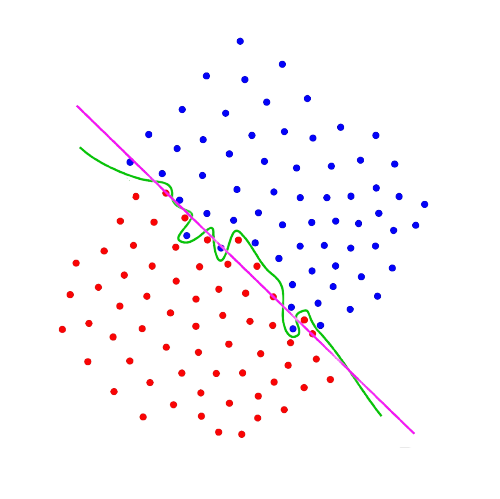
\includegraphics[width=8cm, height=5cm]{overfitting_clean.png}
\caption{Sobreajustament}
\end{figure}

Podem observar que utilitzant el classificador de color verd obtenim una precisió del $100 \%$ a l'hora de classificar les dues categories en la mostra d'entrenament. Tot i això, és molt probable que si utilitzem el classificador amb noves dades independents a la mostra d'entrenament la precisió baixi de manera considerable. Aquest fet es podria haver evitat si en comptes d'usar el classificador verd haguéssim utilitzat el lila, el qual comet més errors en la mostra d'entrenament, però segurament generalitza millor amb noves dades.

Les causes del sobreajustament en models de deep learning poden ser moltes, però dos en les que podríem caure en aquest projecte són:

\begin{enumerate}
    \item Entrenar un model massa complex pot portar a un sobreajustament no desitjat. Una Xarxa Neuronal augmenta en complexitat a mesura que li afegim capes i neurones i, per norma general, com més profunditat més augmenta la capacitat del model de reconèixer patrons en les dades. Malgrat tot si les dades tenen una dimensió reduïda aquest augment en la complexitat ens pot portar a un sobreajustament.
    \item Fer moltes iteracions en els algoritmes d'optimització també és una causa freqüent de sobreajustament. En aquest cas posar un límit en el nombre de vegades que repetim l'algoritme o parar abans d'obtenir valors molt propers a $0$ de la funció de cost ens ajudarà a evitar-lo.
\end{enumerate}

\newpage

\section{Arbres de decisió i Random Forest}

Hem triat els arbres de decisió com a model alternatiu per la seva senzillesa i bons resultats en conjunts de dades amb dimensions i estructura com el que tenim entre mans. En concret, prendrem una variant d'aquests arbres que combina els resultats de diferents models per tal d'evitar el sobreajustament, l'anomenat Random Forest. Però no avancem els esdeveniments, parlem primer de què són els arbres de decisió i de com funcionen.

\subsection{Arbres de decisió}

Els arbres de decisió són models d'aprenentatge automàtic que no pertanyen al subconjunt de l'aprenentatge profund. Són fàcils d'interpretar i d'utilitzar, però no són competitius amb els models de Deep Learning quan tractem amb quantitats enormes de dades. Tot i així en casos amb conjunts de dades més reduïts com el nostre poden ser de gran utilitat.

Els arbres es poden dividir en dues categories segons l'objectiu del problema a resoldre:
\begin{itemize}
    \item \textbf{Arbres de classificació:} 
    La variable que volem predir és categòrica i el model ens retornarà un conjunt de probabilitats per cada una de les categories possibles per cada un dels inputs. Per norma general assignarem la categoria amb la probabilitat més alta a l'input, però podem modificar el marge de decisió per tal d'obtenir resultats més satisfactoris.
    
    \item \textbf{Arbres de regressió:} 
    En aquest cas la variable a predir és contínua i l'objectiu és predir el seu valor, com per exemple predir el preu del metre quadrat dels pisos en diferents zones d'una ciutat.
\end{itemize}

En el nostre cas com que el nostre objectiu és predir si un pacient tindrà o no complicacions ens centrarem en els arbres de classificació. En essència el que fa un arbre de decisió és dividir l'espai predictor en $K$ nodes que anomenarem fulles i cada node es caracteritza per una sèrie de normes. La predicció que retornarà el model per un input concret que compleixi totes les normes d'un node serà la moda d'aquest en la mostra d'entrenament. Aquests models comencen des de dalt dividint l'espai de les observacions en dos de forma binària utilitzant un dels predictors. Una vegada tenim l'espai dividit en dos fem el mateix per cada un dels nous nodes utilitzant un altre predictor i així successivament fins que arribem als nodes inferiors o fulles utilitzant un criteri de parada. El següent esquema il·lustra molt bé com podríem procedir amb les nostres dades i predictors:

\begin{figure}[H]
\label{fig: exemplearbre}
\centering
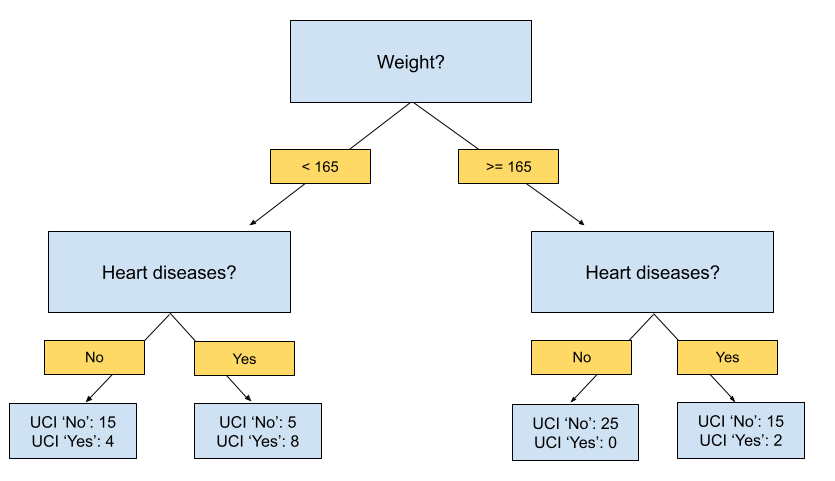
\includegraphics[width=12.5 cm, height = 8 cm]{decision_tree.png}
\caption{Exemple d'arbre}
\end{figure}

En aquest exemple fictici (els resultats no estan basats en la mostra que tenim) veiem que la primera separació binària es fa amb el predictor Weight el qual divideix la mostra en dos conjunts en funció de si el pes és inferior o superior a 165. La segona separació es fa en funció de si els pacients han patit o no problemes cardiovasculars utilitzant el predictor Heart diseases i obtenim els 4 nodes fulla de la part inferior de la figura. Cada un dels nodes conté un nombre $x$ de pacients de la mostra train. En el cas de, per exemple, el primer començant per l'esquerra, tenim 15 pacients que no han tingut simptomatologia greu i 4 que sí complint que el seu pes és menor a 165 i no tenen un historial de malalties cardiovasculars. Per tant, si al nostre arbre li posem com a input un pacient amb un pes de 160 i sense historial de malalties cardiovasculars el model el classificaria com a 'No', ja que és la moda en el node fulla que li pertoca. Aquest arbre el podríem haver fet més profund considerant interaccions amb altres predictors com per exemple en gènere o l'edat.

\subsubsection{Entrenament d'arbres de classificació}

És evident doncs que ens agradaria dissenyar aquests arbres per tal que els nodes fulla fossin tan purs com sigui possible amb relació a la nostra variable a predir. És a dir, seria ideal obtenir nodes fulla tals que tots els seus elements hagin patit complicacions o no les hagin patit. Així, quan li posem a l'arbre un input nou i compleixi les condicions d'un dels nodes fulla que sigui pur, no hi haurà cap dubte de com classificar-lo ja que tots els exemples anteriors pertanyien a una categoria concreta. Per tant, seria força útil tenir això en compte a l'hora de dissenyar el model. El primer pas doncs, serà definir una manera de quantificar com és de pur un node i com podem utilitzar aquesta informació per crear el millor model possible. Tenim diverses opcions depenent novament del nostre objectiu:

\begin{itemize}
    \item \textbf{Error quadràtic o suma dels residus al quadrat RSS:}
    $$RSS = \sum _{i \in A_1}  (y_i - \bar{y}_{A_1})^2 +  \sum _{i \in A_2}  (y_i - \bar{y}_{A_2})^2$$
    On $A_1$ és el primer node de la divisió binària, $A_2$ és el segon node, les $\bar{y}$ són les mitjanes dels valors a predir prenent totes les observacions del node i $y_i$ son els valors reals de la variable resultat.
    
    Notem que una separació perfecta tindria $RSS = 0$ i a mesura que aquest valor creix la separació és cada vegada més dolenta.
    
    \item \textbf{Index Gini:}
    $$G = \sum ^C _{c=1} \hat{p}_{A_1 c} (1-\hat{p}_{A_1 c}) +  \sum ^C _{c=1} \hat{p}_{A_2 c} (1-\hat{p}_{A_2 c}) $$
    
    On $C$ és el nombre de possibles classes en què volem classificar i $\hat{p}_{A_i c}$ és la proporció d'observacions en el node $A_i$ de la classe $c$. Novament en una separació en dos nodes completament purs $G = 0$ i en una separació en dos nodes completament impurs en una classificació binària com la d'aquest projecte (és a dir: els nodes contenen la mateixa proporció de cada una de les classes) tenim:
    $$G = 2 \cdot 0.5 \cdot (1-0.5) + 2 \cdot 0.5 \cdot (1-0.5) = 0.5$$
\end{itemize}

Per tal de fer la divisió més adient utilitzant el predictor més adient i el punt de tall òptim el model cercarà entre tots els predictors diferents punts de tall per calcular les funcions de cost i elegirà a cada pas el predictor i el punt de tall que minimitzin aquesta funció ($RSS$ en cas d'arbres de regressió i Gini en cas de classificació).

\subsection{Arbres de decisió i sobreajustament}

Arribats a aquest punt si continuéssim dividint els nodes podríem arribar a obtenir nodes fulla completament purs els quals només contindrien una sola observació. Aquest arbre tindria un rendiment perfecte a la mostra d'entrenament, però estaria clarament sobreajustat a aquesta mostra i no donaria bons resultats per noves observacions. Per tant, cal especificar un criteri de parada per tal que l'arbre no creixi massa profund. Tres bons criteris que s'acostumen a utilitzar junts són els següents:

\begin{itemize}
    \item Per una banda podem especificar un nombre mínim d'observacions que ha de tenir un node per tal de dividir-lo en dos nodes fills. Aquest valor dependrà molt de la quantitat de dades amb les quals estiguem tractant, ja que per conjunts més petits de dades es permeten valors més petits per aquest paràmetre.
    \item Per altra banda podem definir una profunditat màxima que pot assolir l'arbre per tal d'estalviar-nos complexitat 
    \item També podem decidir no dividir un dels nodes en cas que no millori el model de manera significativa. És a dir, el millor resultat obtingut en les funcions de cost és massa gran i no val la pena introduir complexitat al model per la poca recompensa que obtenim.
\end{itemize}

Aquestes estratègies acostumen a funcionar força bé, però com ja hem dit la capacitat predictiva dels arbres és moderada. És per això que s'han proposat mètodes que combinen el resultat de diversos arbres de decisió per millorar el poder predictiu dels models.

\subsection{Models Random Forest}

Un d'aquests models que combinen l'output de diversos arbres és l'anomenat Random Forest. El principi fonamental darrere aquests algoritmes és utilitzar un conjunt de models mediocres per aconseguir un model molt més efectiu. Introduirem dues noves estratègies:

\begin{itemize}

\item La primera que utilitzarem per a reduir la variància és entrenar diferents arbres amb subconjunts de dades de la mostra d'entrenament i calcular la mitjana dels resultats de tots els arbres en cas d'arbres de regressió i la moda en cas de classificació.

\item La segona estratègia que seguirem és que per cada una de les divisions de nodes que considerem fer dins dels arbres només considerem una mostra aleatòria d'entre el total dels nostres predictors de mida $m$. Per norma general si $p$ és el nombre total de predictors s'acostuma a prendre $m \approx \sqrt{p}$

\end{itemize}

El nombre d'arbres a entrenar encara és tema de discussió, però tot indica que el rendiment empitjora a l'utilitzar massa arbres i per norma general provarem amb valors al voltant de $500$. \\

El següent esquema il·lustra molt bé com aquest algoritme a l'hora de fer prediccions:

\begin{figure}[H]
\label{fig: esquemaRF}
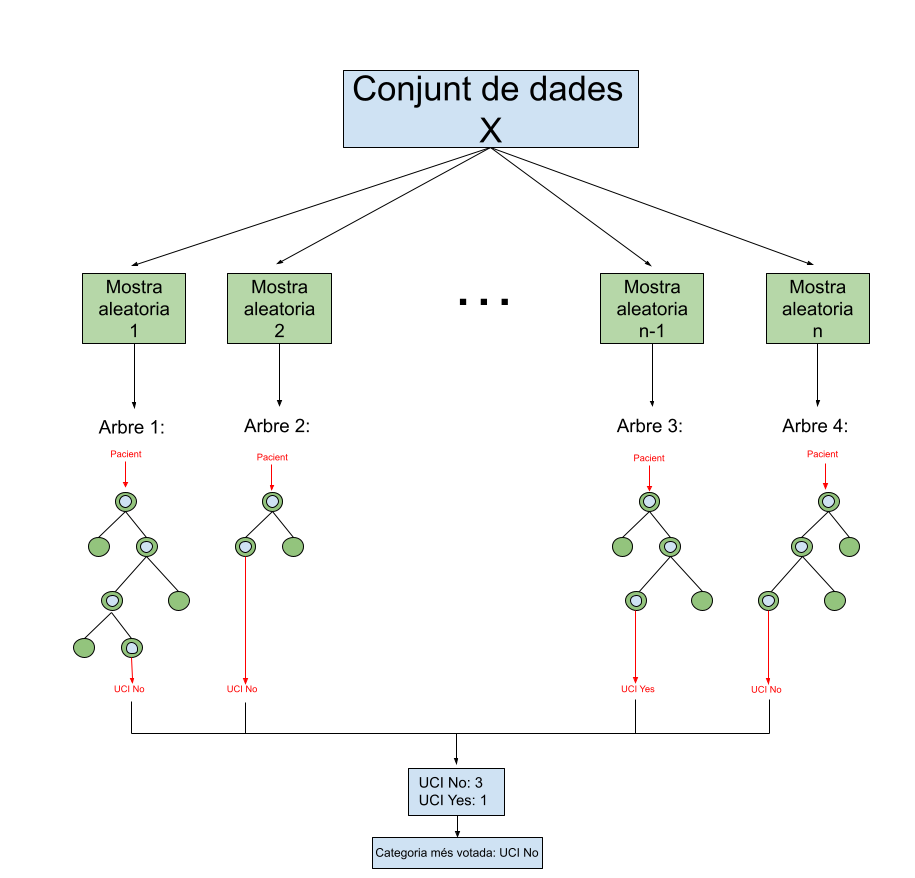
\includegraphics[width=13.8 cm, height = 12 cm]{random_forest.png}
\caption{Esquema Random Forest}
\end{figure}

Els nodes amb el cercle blau dins representen el camí que ha seguit el pacient per cada un dels arbres fins a arribar a l'output. En el nostre cas, com que la variable que volem predir és binària ens quedarem amb la moda de tots els outputs.

\newpage

\section{Introducció a la base de dades, objectius i anàlisi}

La base de dades de la que disposem conté la informació d'exactament $2283$ pacients de l'hospital clínic de Barcelona i, com ja hem exposat al principi de la memòria, el nostre objectiu és crear un algoritme de Deep Learning utilitzant xarxes neuronals capaces de predir la severitat dels símptomes de la COVID-19 en pacients. Considerarem que un pacient positiu de COVID-19 ha patit símptomes severs de la malaltia en cas que hagi estat ingressat a la Unitat de Cures Intensives (UCI). \\

Les dades contenen informació dels pacients sobre els següents camps:

\begin{enumerate}
    \item \textbf{ID:} Número d'identificació del pacient.
    \item \textbf{UCI:} Variable binària que indica si el pacient ha patit símptomes greus en contagiar-se de COVID-19.
    \item \textbf{Age:} Edat del pacient.
    \item \textbf{Gender:} Gènere del pacient.
    \item \textbf{Size:} Talla del pacient.
    \item \textbf{Weight:} Pes del pacient.
    \item \textbf{Size\_mt:} Talla del pacient dividida entre 10.
    \item \textbf{IMC:} Index de massa corporal.
    \item \textbf{BW:} Pes del pacient al neixer.
    \item \textbf{BW\_2500:} Variable binària que indica si el pacient va néixer amb un pes anormalment baix. Considerem un pes anormalment baix aquells pacients amb pesos iguals o inferiors a $2500$ grams.
    \item \textbf{Percentil\_birth:} Percentil de naixement.
    \item \textbf{IUGR\_calc:}  Variable binària que indica si el pacient ha patit Restricció del Creixement Intrauterí (Intrauterine Growth Restriction)
    \item \textbf{Tobacco\_yes\_no:} Variable binària que indica si l'hàbit de fumar ha estat present en la vida del pacient.
    \item \textbf{Hipertension:} Variable binària que indica si el pacient ha patit o pateix hipertensió.
    \item \textbf{Heart\_diseases:} Variable binària que indica si el pacient ha patit o pateix malalties cardiovasculars.
    \item \textbf{DM:} Variable binària que indica si el pacient ha patit o pateix diabetis.
    \item \textbf{Dyslipidemia:} Variable binària que indica si el pacient ha patit o pateix dislipidèmia.
    \item \textbf{Obesity:} Variable binària que indica si el pacient ha patit o pateix obesitat.
    \item \textbf{Kidney\_disease:} Variable binària que indica si el pacient ha patit o pateix malalties relacionades amb els ronyons.
    \item \textbf{Autoimmune:} Variable binària que indica si el pacient ha patit o pateix malalties de caràcter autoimmune.
    \item \textbf{Cancer:} Variable binària que indica si el pacient ha patit o pateix algun tipus de càncer.
    \item \textbf{Thyroid:} Variable binària que indica si el pacient ha patit o pateix malalties de tiroides.
    \item \textbf{Infectious:} Variable binària que indica si el pacient ha patit o pateix malalties de caràcter infecciós.
    \item \textbf{Psychiatric:} Variable binària que indica si el pacient ha patit o pateix malalties psiquiàtriques.
\end{enumerate}

Una vegada enumerats tots els nostres predictors ja podem començar amb l'exploració d'aquests. El primer que farem és visualitzar la distribució de la variable més important i aquella que volem predir. La variable UCI:

\begin{figure}[H]
\label{fig: UCIdist}
\centering
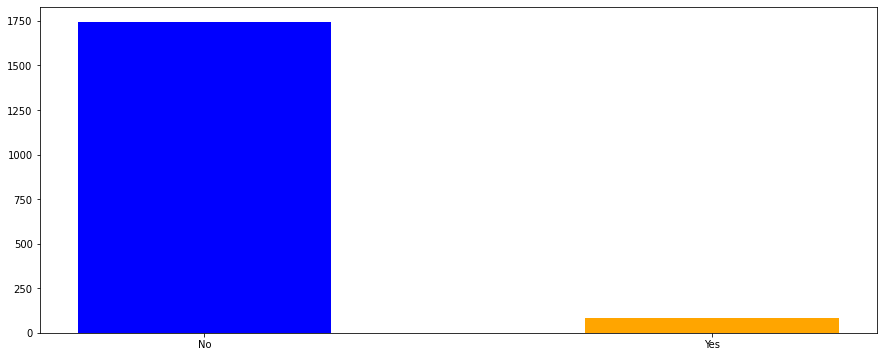
\includegraphics[width=12.2 cm, height = 5 cm]{unbalanced_data.png}
\caption{Distribució de UCI}
\end{figure}

Com ja esperàvem les dades estan fortament des-balancejades, és per això que per entrenar els nostres models provarem tècniques de balanceig de dades per veure si els algoritmes tenen un millor rendiment amb aquestes modificacions.

Seguim veient la distribució de l'edat i el pes:

\begin{figure}[H]
\label{fig: ageweightdist}
\centering
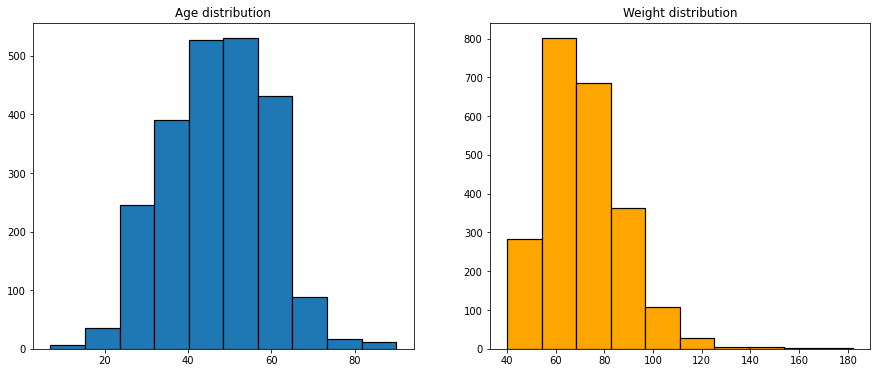
\includegraphics[width=12.2 cm, height = 5 cm]{age_weight_dist.png}
\caption{Distribució d'edat i pes}
\end{figure}

Podem veure que les dades estan força ben distribuïdes entre les edats de 25 i 65. Per tant, tenim una bona mostra estadística amb relació a l'edat. En el cas del pes tenim una mitjana al voltant dels 70. Obtindrem més informació sobre aquesta variable dividint entre homes i dones. Farem el mateix amb el IMC: \\

\begin{figure}[H]
\label{fig: genderweightIMCdist}
\centering
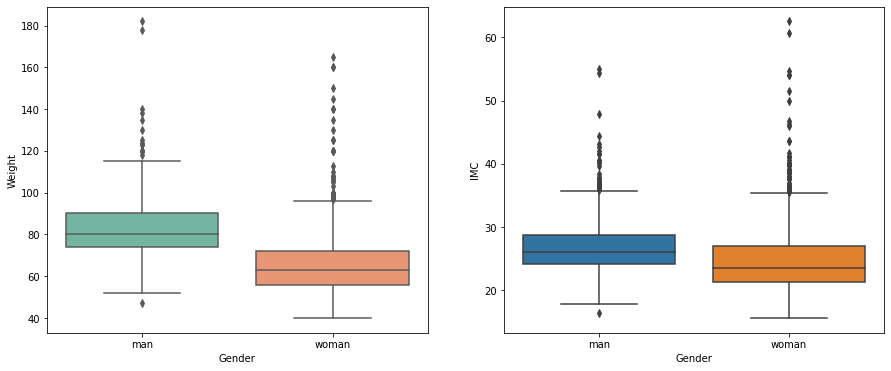
\includegraphics[width=12.2 cm, height = 5 cm]{boxplot_weight_IMC.png}
\caption{Distribució d'edat i pes}
\end{figure}

Com ja esperàvem, podem veure un augment en la variable pes en el cas del gènere masculí. Observem que la mitjana del pes en homes està per sobre dels 80 kg que és una mica més alt que la mitjana de pes a Espanya. Aquest fenomen és degut al fet que la nostra base de dades recull una mostra d'edat més avançada. El mateix passa amb el gènere femení. \\

També volem estudiar les relacions que hi ha entre predictors i no només la relació dels predictors amb la variable a predir. Començarem explorant l'impacte que podria tenir en el pes durant l'edat adulta el fet d'haver patit complicacions durant l'embaràs com pot ser un pes anormalment baix o haver patit restricció del creixement intrauterí.

\begin{figure}[H]
\label{fig: BWIUGR}
\centering
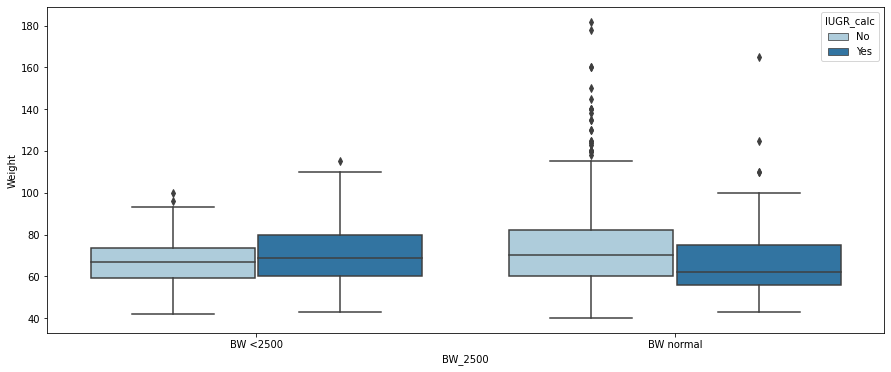
\includegraphics[width=12.2 cm, height = 5 cm]{boxplot_BW_IUGR.png}
\caption{Funcionament d'una neurona}
\end{figure}

Observem que aquells pacients que tenen un BW normal però que sí que van patir IUGR tendeixen a tenir un pes més baix en l'etapa adulta. En el cas d'aquells pacients que no han patit IUGR aquells que van néixer amb un pes anormalment més baix tendeixen a tenir també un pes més baix a l'etapa adulta. En el cas dels que sí que van néixer amb un pes inferior a $2500$ grams veiem que, sorprenentment, la mitjana del pes augmenta en els que van patir IUGR però no de forma significativa.

\subsection{Impacte de les variables categòriques sobre la variable UCI}

Vegem primer quina relació tenen les variables categòriques com Obesity o Psychiatric sobre la nostra variable a predir:

\begin{figure}[H]
\label{fig: categUCI}
\centering
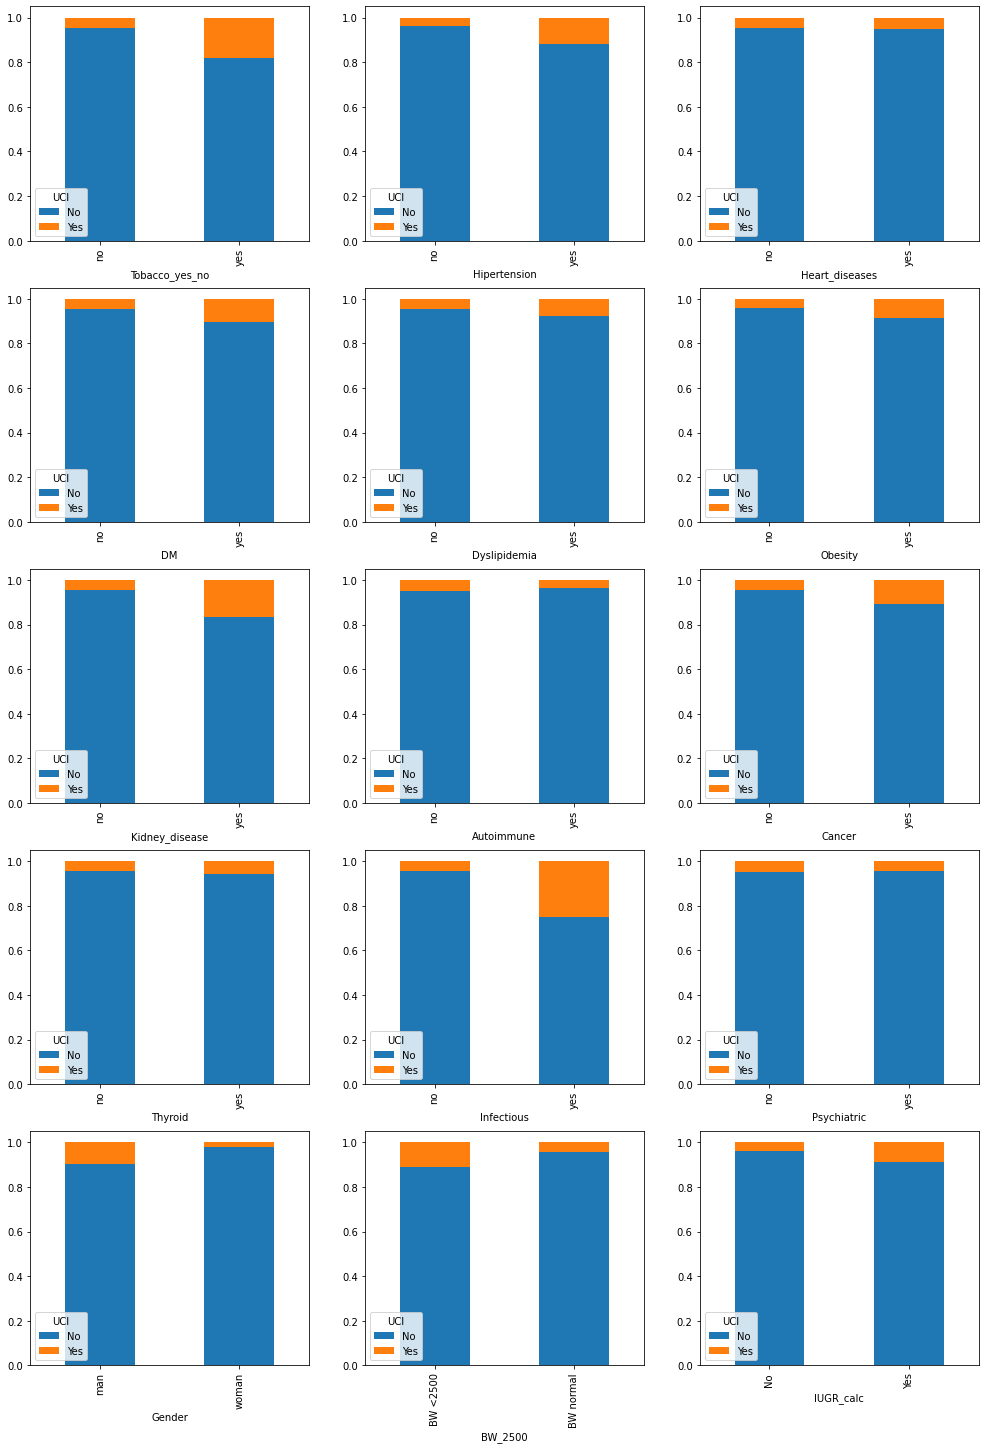
\includegraphics[width=13 cm, height = 18 cm]{categ_and_UCI.png}
\caption{Variables categòriques i UCI}
\end{figure}

Aquests gràfics ens mostren els percentatges dels pacients amb simptomatologia greu dividits en dues mostres segons la variable categòrica que apareix a la part inferior del gràfic. \\

Definirem tres categories diferents: Considerarem que una malaltia, una condició o un hàbit té un fort impacte en la probabilitat de patir conseqüències greus si el fet de patir-la, haver-la patit o haver practicat aquell hàbit fa que aquesta probabilitat sigui igual o superior a $0.15$. Considerarem que el predictor té un impacte moderat si la probabilitat és més petita que $0.15$ i més gran o igual que $0.08$. Finalment, considerarem que no hi ha cap relació aparent, o en altres paraules no tenim evidència estadística suficient d'una relació, si la probabilitat és més petita que $0.08$.

Amb aquestes categories ben definides doncs podem extreure les següents conclusions:

\begin{enumerate}
    \item El \textbf{consum de tabac}, les \textbf{malalties de ronyons} i les \textbf{malalties infeccioses} tenen un \textbf{fort impacte} en la probabilitat de patir símptomes greus de la malaltia.
    \item La \textbf{hipertensió}, la \textbf{diabetis}, la \textbf{obesitat}, el \textbf{càncer} i la \textbf{restricció del creixement intrauterí} tenen un \textbf{impacte moderat} en la probabilitat de patir símptomes greus de la malaltia.
    \item No trobem una relació aparent entre la variable UCI i el fet d'haver patit o patir \textbf{malalties cardiovasculars}, \textbf{dislipidèmia}, \textbf{malalties autoimmunes}, \textbf{tiroides} i \textbf{malalties psiquiàtriques}.
\end{enumerate}

Per altra banda, si analitzem les variables de pes al néixer i el gènere trobem dos fets força interessants:
\begin{enumerate}
    \item Un baix pes al néixer podria duplicar la probabilitat de patir símptomes greus.
    \item Els homes són 5 vegades més propensos a patir simptomatologia greu.
\end{enumerate}

Cal tenir en compte que verificarem aquests enunciats utilitzant un mapa de correlacions més endavant per assegurar-nos que aquestes són estadísticament significatives.

\subsection{Correlació entre les variables contínues}

Vegem, per ser exhaustius, la correlació entre les variables contínues amb un mapa de correlacions:

\begin{figure}[H]
\label{fig: corrcont}
\centering
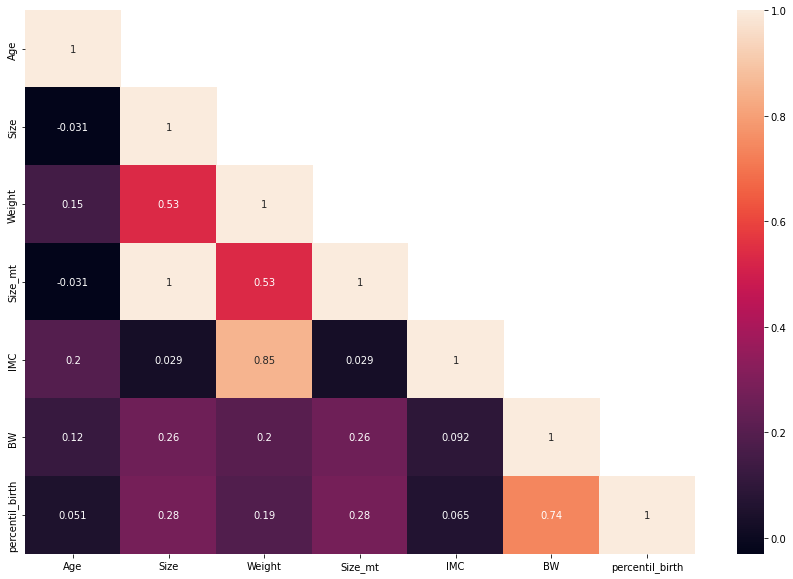
\includegraphics[width=12.2 cm, height = 7 cm]{corr_cont.png}
\caption{Correlació variables contínues}
\end{figure}

Trobem algunes relacions que ja esperàvem com:

\begin{itemize}
    \item \textbf{Weight} amb \textbf{Size}
    \item \textbf{Weight} i \textbf{IMC}
    \item \textbf{percentile\_birth} i el \textbf{BW}
\end{itemize}

Estudiarem també l'impacte que tenen l'edat i el pes sobre UCI:

\begin{figure}[H]
\label{fig: weightageUCI}
\centering
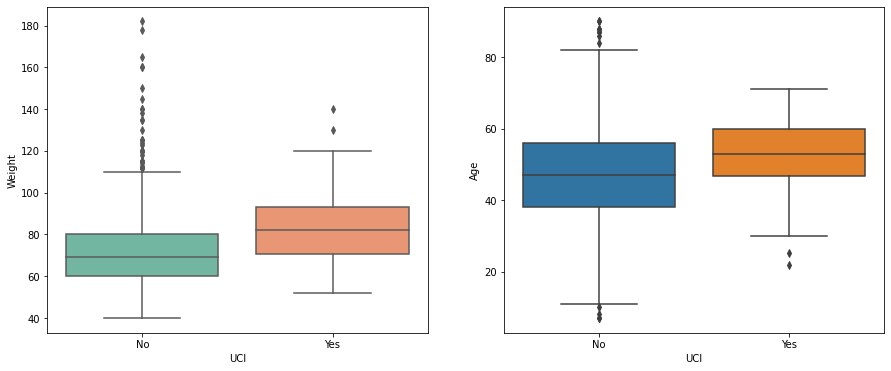
\includegraphics[width=13 cm, height = 5.5 cm]{UCI_age_weight.png}
\caption{Pes i edat amb UCI}
\end{figure}


En tots dos casos podem veure que hi ha un lleuger increment tant en pes com en edat en els pacients que han patit simptomatologia greu.

\subsection{Chi test}

Com ja hem dit ens agradaria tenir una manera de verificar els impactes de les variables categòriques sobre UCI. El candidat serà el chi-test de la llibreria scipy.stats que ens retornarà els p-valors de les relacions entre cada una de les variables i d'aquesta manera podrem afirmar si hi ha o no relació:

Considerarem que un p-valor més petit de $0.05$ és suficient per rebutjar la hipòtesi nul·la i afirmar que les variables estan correlacionades:

\begin{figure}[H]
\label{fig: pvaluesheatmap}
\centering
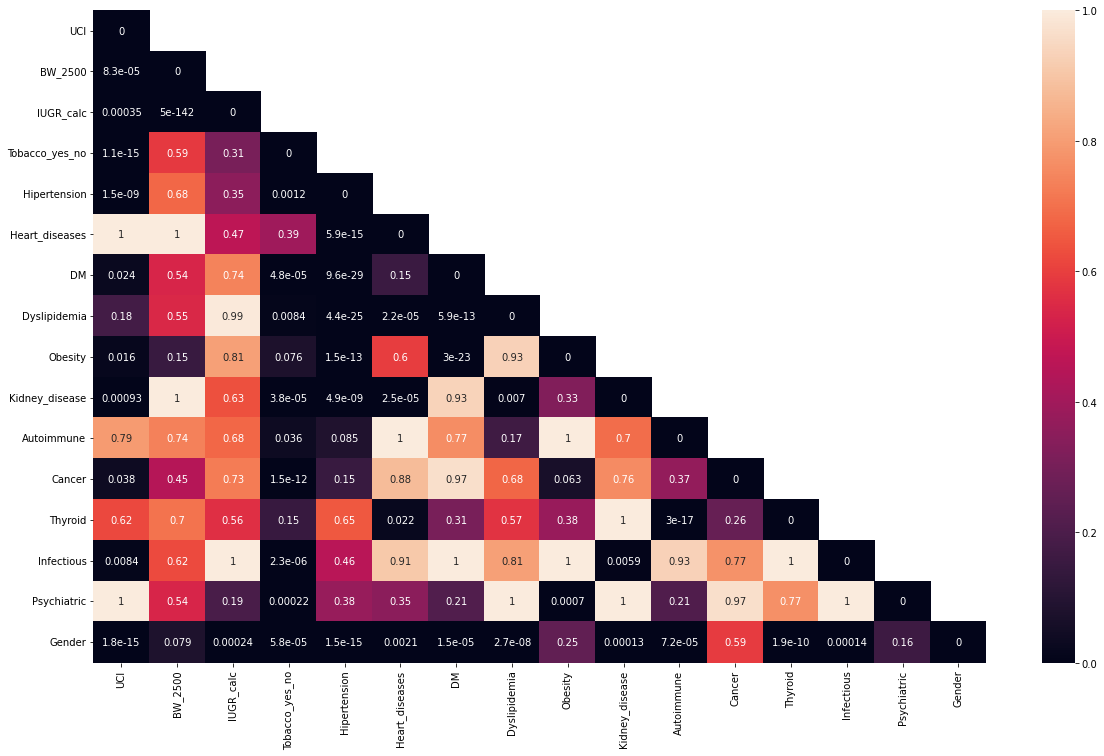
\includegraphics[width=12.2 cm, height = 9 cm]{p-values_heatmap.png}
\caption{p-valors}
\end{figure}


Aquest mapa ens confirma a la perfecció les hipòtesis de correlació que hem plantejat a la secció 7.1. Si ens fixem en els p-valors, aquells que són més grans que la cota que hem marcat són d'aquells predictors que hem intuït que no tenien cap relació aparent amb UCI. Per altra banda, les variables que tenen un impacte fort o moderat són aquelles amb p-valors superiors a $0.05$. Per tant, podem dir que hem verificat estadísticament totes les nostres hipòtesis.

\section{Resultats amb Xarxes Neuronals}

Proposem utilitzar un model de Deep Learning amb xarxes neuronals amb les següents característiques:

\begin{enumerate}
    \item batch\_size = 50 en les dades d'entrenament
    \item Funció d'activació ReLU en la capa intermèdia i activació Softmax en l'última capa
    \item Epochs = 10
    \item Funció de cost: Entropia creuada categòrica
    \item Optimitzador: ADAM
    \item Paràmetre d'aprenentatge $\eta = 0.0001$
\end{enumerate}

Hem entrenat el model utilitzant acceleració CPU per motius de velocitat. Obtenim els següents valors de la funció de cost pels 4 últims epochs:

\begin{table}[h]
\begin{tabular}{|l|l|l|l|l|}
\hline
\textbf{Epochs:}   & 7     & 8     & 9     & 10    \\ \hline
\textbf{nll\_loss} & -0.96 & -0.99 & -0.99 & -0.88 \\ \hline
\end{tabular}
\end{table}

Clarament, el model s'ajusta terriblement a les dades d'entrenament i, si fem prediccions, el model classifica tots els elements de la mostra test com a $0$ (Codificació en el tensor per UCI = No). Aquest resultat pot ser causat per la falta de pacients a la mostra train amb UCI = Sí. Intentarem sortejar aquest fet utilitzant una mostra remostrejada amb la tècnica upsampling, que consisteix a replicar dades de pacients amb UCI = Sí per tal de balancejar les dues categories, amb l'esperança que aquesta doni millors resultats. \\

En aquest cas utilitzarem una estratègia lleugerament diferent. Dividirem les nostres dades en tres mostres:

\begin{enumerate}
    \item \textbf{Train:} Dades que utilitzarem per a l'entrenament del model.
    \item \textbf{Validation:} Dades que utilitzarem per determinar l'hiperparàmetre prob. Aquest serà el que determinarà el llindar de decisió de la probabilitat en els resultats.
    \item \textbf{Test:} Dades que utilitzarem per comprovar com funciona el model en dades independents.
\end{enumerate}

Obtenim els següents resultats per els 4 últims epochs:

\begin{table}[h]
\begin{tabular}{|l|l|l|l|l|}
\hline
\textbf{Epochs:}   & 7     & 8     & 9     & 10    \\ \hline
\textbf{nll\_loss} & -0.29 & -0.40 & -0.43 & -0.30 \\ \hline
\end{tabular}
\end{table}

Observem que en aquest cas el model s'ajusta molt millor a les dades d'entrenament. Si fem unes prediccions en aquest moment amb el marge $prob=0.5$ que és el que s'utilitza per defecte com en el cas anterior el model prediu tots els pacients com a 'No'. Fem prediccions ara amb el conjunt de dades de validació per ajustar prob:

\ 

Explorant $2000$ possibles valors per prob obtenim els millors resultats amb prob $=0.99994$. Si utilitzem ara aquest valor per calcular prediccions sobre la mostra test obtenim:

\begin{table}[h]
\begin{tabular}{|l|l|}
\hline
\textbf{Precisió No} & \textbf{Precisió Si} \\ \hline
0.95        & 0.00                 \\ \hline
\end{tabular}
\end{table}

El model continua tenint un rendiment molt pobre en dades independents a l'entrenament.

Com que amb les dades remostrejades disposem de més volum de pacients afegirem dues capes més de profunditat a la xarxa i estudiarem els resultats:

Els 4 últims epochs:

\begin{table}[h]
\begin{tabular}{|l|l|l|l|l|}
\hline
\textbf{Epochs:}   & 7     & 8     & 9     & 10    \\ \hline
\textbf{nll\_loss} & -0.53 & -0.55 & -0.51 & -0.57 \\ \hline
\end{tabular}
\end{table}

ajustem l'hiperparàmetre $prob$ de la mateixa manera i obtenim:

\begin{table}[h]
\begin{tabular}{|l|l|}
\hline
\textbf{Precisió No} & \textbf{Precisió Si} \\ \hline
0.95        & 0.00                 \\ \hline
\end{tabular}
\end{table}

Una xarxa més profunda no aconsegueix millorar els resultats. 


\section{Resultats amb Random Forest}

Per entrenar els models hem triat la llibreria H2O per la seva versatilitat i adaptabilitat als conjunts de dades que combinen dades categòriques i continues com és el nostre cas. La nostra estratègia consistirà a entrenar una gran quantitat de models amb diferents combinacions d'hiperparàmetres i utilitzant un subconjunt de les dades que anomenarem conjunt test anirem validant els models per triar finalment el que considerem que té millor rendiment seguint els punts que ja hem especificat (Recordem que ens hem marcat com a principal objectiu obtenir una precisió molt alta sobre els negatius sacrificant si és oportú la precisió en els positius). \\

Cal remarcar que la llibreria H2O no utilitza arbres de classificació per a afrontar problemes de classificació com el nostre sinó que sempre utilitza arbres de regressió, transformant les variables categòriques en continues. Aclarit aquest fet procedim a presentar els models i resultats:\\

El primer pas ha estat dividir les nostres dades en un conjunt d'entrenament ($80\%$ del total) i un conjunt de validació ($20\%$ restant). Ja hem comentat que disposem d'unes dades molt desbalacejades així que hem optat per provar dos enfocaments diferents:

\begin{itemize}
    \item El primer serà entrenar els models amb la mostra de dades train tal com la tenim.
    \item El segon consistirà a utilitzar la tècnica de remostreig upsampling i utilitzar les noves dades per entrenar un nou model.
\end{itemize}

Comencem amb el primer enfocament:

Per tal d'explorar totes les possibilitats hem entrenat un model per cada una de les combinacions possibles dels següents hiperparàmetres:

\begin{itemize}
    \item Nombre d'arbres: $500$, $600$ o $700$
    \item Màxima profunditat: $3$, $4$, $5$, $6$ o $7$
    \item Mínim d'observacions per node: $6$, $10$, $15$ o $20$
\end{itemize}

També explorarem diversos marges de decisió a l'hora de classificar les nostres categories per trobar l'òptim. Obtenim els següents models guanyadors:

\begin{table}[H]
\begin{tabular}{llll}
\hline
\multicolumn{1}{|l|}{\textbf{Identificador}} & \multicolumn{1}{l|}{Num. arbres} & \multicolumn{1}{l|}{Màx. profunditat} & \multicolumn{1}{l|}{Mín. node} \\ \hline
gbm\_grid1\_model\_55                        & 700                                & 7                                     & 15                             \\
gbm\_grid1\_model\_35                        & 600                                & 7                                     & 15                             \\
gbm\_grid1\_model\_15                        & 500                                & 7                                     & 15                            
\end{tabular}
\end{table}

\begin{table}[H]
\begin{tabular}{llll}
\hline
\multicolumn{1}{|l|}{\textbf{Identificador}} & \multicolumn{1}{l|}{Marge} & \multicolumn{1}{l|}{Precisió No} & \multicolumn{1}{l|}{Precisió Si} \\ \hline
gbm\_grid1\_model\_55                        & 0.925                      & 0.99                             & 0.2                              \\
gbm\_grid1\_model\_35                        & 0.925                      & 0.99                             & 0.2                              \\
gbm\_grid1\_model\_15                        & 0.925                      & 0.99                             & 0.2                             
\end{tabular}
\end{table}

Tots tres models tenen els mateixos resultats, però elegirem el tercer pel principi de parsimònia, ja que és el més simple. \\

Amb aquests resultats al cap entrenarem ara els mateixos models però utilitzant la mostra remostrejada amb la tècnica upsampling. Obtenim un sol model guanyador:

\begin{table}[H]
\begin{tabular}{llll}
\hline
\multicolumn{1}{|l|}{\textbf{Identificador}} & \multicolumn{1}{l|}{Num. arbres} & \multicolumn{1}{l|}{Màx. profunditat} & \multicolumn{1}{l|}{Mín. node} \\ \hline
gbm\_grid1\_model\_54                        & 700                              & 6                                     & 15                            
\end{tabular}
\end{table}

\begin{table}[H]
\begin{tabular}{llll}
\hline
\multicolumn{1}{|l|}{\textbf{Identificador}} & \multicolumn{1}{l|}{Marge} & \multicolumn{1}{l|}{Precisió No} & \multicolumn{1}{l|}{Precisió Si} \\ \hline
gbm\_grid1\_model\_54                        & 0.5                        & 0.98                             & 0.19                            
\end{tabular}
\end{table}

Observem que els resultats no només no milloren sinó que són lleugerament pitjors. Per tant, concloem que el model que millor satisfà les nostres necessitats és l'identificat com  gbm\_grid1\_model\_15. 

\newpage

\section{Resultats, conclusions i possibles ampliacions}

Si comparem els millors resultats dels dos models:

\begin{table}[h]
\begin{tabular}{l|l|l|l|}
\cline{2-4}
                            & \textbf{Model}        & \textbf{Precisió Si} & \textbf{Precisió No} \\ \hline
\multicolumn{1}{|l|}{Xarxa} & network               & 0.0                  & 0.95                 \\ \hline
\multicolumn{1}{|l|}{RF}    & gbm\_grid1\_model\_15 & 0.2                  & 0.99                 \\ \hline
\end{tabular}
\end{table}

Tenim un claríssim guanyador. El model basat en arbres Random Forest té un rendiment en la mostra test molt millor que la xarxa neuronal. Els resultats que hem obtingut amb aquesta última han sigut molt deficients i a continuació exposem les possibles causes i conclusions a les quals hem arribat amb relació a la comparació dels models:

\begin{enumerate}[(I)]
    \item La mostra és massa petita per l'entrenament d'una xarxa neuronal. Els models de Deep Learning estan dissenyats per reconèixer patrons en estructures extremadament complexes i, per tal de comprendre aquestes estructures, cal entrenar-les amb conjunts de dades prou grans.
    \item Per norma general els models de Deep Learning són famosos per resoldre problemes amb dades no rectangulars. Entenem com a dades rectangulars aquelles dades tals que les seves columnes o predictors són de naturalesa diferent. Utilitzant aquesta definició les nostres dades són clarament un conjunt rectangular i, per tant, els models basats en xarxes neuronals tindran una capacitat predictiva bastant deficient \footnote{Léo Grinsztajn, Edouard Oyallon, Gaël Varoquaux. Why do tree-based models still outperform deep learning on tabular data?. 2022. ⟨hal-03723551⟩ \url{https://hal.archives-ouvertes.fr/hal-03723551}}.
    \item Els models que hem entrenat amb xarxes semblen tenir una predisposició a classificar tots els pacients de la mostra test amb l'etiqueta $0$ (categoria 'No' codificada) probablement causada pel desbalancejament de les dades.
    \item La tècnica de balanceig de dades upsampling no sembla tenir cap efecte en el rendiment de la xarxa degut a que la repetició de dades no aporta informació nova al model
    \item L'augment de la profunditat de la xarxa, i per conseqüència de la complexitat, no ha portat millores significatives en les prediccions. Descartem doncs que el fracàs en les prediccions sigui causat per entrenar una xarxa poc profunda. Degut a la dimensió de les dades i a la naturalesa del problema no cal afegir complexitat al model de forma innecessària.
    \item Sobre el model de Random Forest l'augment d'arbres no millora el model de manera significativa. Per tant, com en el punt anterior, afegir complexitat no ens proporciona millors resultats pel mateix motiu.
    \item Novament, com amb les xarxes, entrenar el model RF amb les dades remostrejades no millora les prediccions. Tot i això, remarquem que per obtenir pràcticament els mateixos resultats ha calgut afegir complexitat al model (200 arbres).
    \item El model RF té un rendiment força superior a totes les xarxes neuronals que hem implementat. Podem concloure doncs que per fer prediccions sobre simptomatologia associada al COVID-19 utilitzant els predictors dels quals disposem els models Random Forest ofereixen prediccions molt més precises i fiables.
\end{enumerate}

\subsection{Resultats pràctics}

Si recordem, al principi d'aquest projecte, hem justificat els motius pels quals hem prioritzat la precisió sobre els pacients amb UCI = 'No', sacrificant d'aquesta manera precisió en aquells amb UCI = 'Sí'. Estudiarem a fons els resultats obtinguts amb el model de Random Forest gbm\_grid1\_model\_15, ja que ha sigut el que millor satisfà els nostres requisits:

\begin{enumerate}[(I)]

\item El model només prediu 4 falsos negatius (Pacients tals que es prediu UCI='No' però el valor real és UCI='Sí') que representa un 1 \% de tots els pacients que hem predit que no patiran simptomatologia greu (355). És a dir, el model permet pràcticament eliminar el risc de complicacions en la malaltia en pacients descartats.
\item El 84 \% de tots els pacients de la mostra test que patiran símptomes greus han estat correctament classificats. $21$ classificacions exitoses d'un total de $25$.
\item Per tal d'assolir aquests resultats es prediuen $102$ pacients com a UCI='Sí' dels quals $21$ són realment UCI='Sí' que es tradueix en una proporció del 20 \%
\item Es cometen 81 falsos positius (Pacients tals que es prediu UCI='Sí' però el valor real és UCI='No') que representa un 80\% de tots els pacients classificats amb UCI='Sí'. Aquest resultat no és alarmant en absolut, ja que són pacients que no patiran complicacions.
\end{enumerate}

\subsection{Possibles ampliacions}
Una de les raons per les quals no hem obtingut tan bons resultats com ens hauria agradat ha sigut per la reduïda dimensió de les dades de les quals disposem. Seria interessant recollir les dades d'un conjunt del voltant de 10000 pacients amb les mateixes variables per estudiar si el model Random Forest obté millors resultats amb un conjunt més ampli. Per altra banda, és conegut que els models de Boosting són excel·lents a l'hora de fer prediccions amb dades rectangulars, com és el nostre cas. Una possible ampliació seria ajustar un d'aquests models a les nostres dades i comparar els resultats amb els assolits amb RF en aquest projecte.

\newpage

\section{Respositoris}

\begin{itemize}
    \item Codi font latex: \url{https://github.com/BetriuJaume/TFG-Latex-code-and-images/tree/main}
    \item Codi python: \url{https://github.com/BetriuJaume/TFG-code}
\end{itemize}

\newpage

\begin{thebibliography}{100} 
\bibitem{AA1} Juan R González.  \emph{Aprendizaje Automático 1}. Grau d'estadística UAB. (2021) \url{https://isglobal-brge.github.io/Aprendizaje_Automatico_1/index.html}

\bibitem{AA2} Roger Borràs. \emph{Aprenentatge Automàtic 2}. Grau d'estadística UAB. (2021)

\bibitem{DLpy} François Chollet. \emph{Deep learning with Python}. Manning Publications Co. (2018)

\bibitem{Ruder} Sebastian Ruder. \emph{An overview of gradient descent optimisation algorithms}. arXiv preprint arXiv:1609.04747. (2016) \url{https://ruder.io/optimizing-gradient-descent/index.html#rmsprop}

\bibitem{Brownlee} Jason Brownlee. \emph{Loss and Loss Functions for Training Deep Learning Neural Networks}. Deep Learning Performance a Machine Learning Mastery. (2019) 

\bibitem{RFvsNN} Léo Grinsztajn, Edouard Oyallon, Gaël Varoquaux. \emph{Why do tree-based models still outperform deep learning on tabular data?}. ⟨hal-03723551⟩, (2022). \url{https://hal.archives-ouvertes.fr/hal-03723551}
\end{thebibliography}


\newpage


\end{document}